%\documentclass{sig-alternate-05-2015}
%\documentclass[10pt,conference]{IEEEtran}
\documentclass{llncs}

\let\proof\relax
\let\endproof\relax
\let\example\relax
\let\endexample\relax

\usepackage[margin=1.5in]{geometry}
\usepackage{makeidx}
\usepackage{tabularx,colortbl}
\usepackage[dvipsnames]{xcolor}
\usepackage{flushend}
\usepackage{cite}
\usepackage{amsmath}
\usepackage{amsthm}
\usepackage{amssymb}
\usepackage{bm}
\usepackage{epsfig}
\usepackage{stmaryrd}
\usepackage{url}
\usepackage{multirow}
\usepackage{latexsym}
\usepackage{graphics}
\usepackage{graphicx}
\usepackage{enumitem}
\usepackage{comment}
\usepackage{longtable}
\usepackage{supertabular}
\usepackage{times}
\usepackage{listings}
\usepackage{subfigure}
\usepackage{booktabs}
\usepackage{color}
\usepackage{balance}
\usepackage{xspace}
\usepackage{hyperref}
\usepackage[ruled, vlined, linesnumbered]{algorithm2e}
\usepackage[autostyle]{csquotes}
\usepackage[]{algorithm2e}
\usepackage{IEEEtrantools}
%\usepackage{fourier} 
\usepackage{array}
\usepackage{makecell}


%\theoremstyle{Definition}
%\newtheorem{definition}{Definition}
%%%
%\theoremstyle{Theorem}
%\newtheorem{theorem}{Theorem}


%\newcommand{\definition}{\noindent \textbf{Definition} \citation{}}
%\newcommand{\theorem}{\noindent \textbf{Theorem} \citation{}}
%\newcommand{\lemma}{\noindent \textbf{Lemma} \citation{}}

%\newdef{lemma}{Lemma}
%\newdef{definition}{Definition}
%\newdef{theorem}{Theorem}
%\newdef{corollary}{Corollary}
%\newdef{note}{Note}
%\newdef{axiom}{Axiom}

%\newtheorem{theorem}{Theorem}
%\newtheorem{definition}{Definition}

\newcommand{\mkeyword}[1]{\mbox{\texttt{#1}}}
\DeclareMathOperator{\kuop}{uop}
\DeclareMathOperator{\kbop}{bop}
\DeclareMathOperator{\kite}{ite}
\DeclareMathOperator{\kpre}{pre}
\DeclareMathOperator{\dom}{dom}
\DeclareMathOperator{\ktrue}{true}
\DeclareMathOperator{\kfalse}{false}
\DeclareMathOperator{\kselect}{select}
\DeclareMathOperator{\ran}{range}
\newcommand{\lbb}{[\![}
\newcommand{\rbb}{]\!]}
\newcommand{\jkind}{\texttt{JKind}\xspace}
\newcommand{\lustre}{\texttt{Lustre}\xspace}
\newcommand{\agree}{\texttt{AGREE}\xspace}
\newcommand{\ivc}{\textit{IVC}\xspace}
\newcommand{\unsat}{\texttt{UNSAT}\xspace}
\newcommand{\sat}{\texttt{SAT}\xspace}
\newcommand{\aivcalg}{\texttt{\small{All\_MIVCs}}\xspace}
\newcommand{\amcs}{\texttt{\small{All\_MCSs}}\xspace}

\renewcommand\theadalign{bc}
\renewcommand\theadfont{\bfseries}
\renewcommand\theadgape{\Gape[4pt]}
\renewcommand\cellgape{\Gape[4pt]}

\newcommand{\danielle}[1]{\textcolor{orange}{#1}}
\newcommand{\mats}[1]{\textcolor{blue}{#1}}
\newcommand{\mike}[1]{\textcolor{red}{#1}}
\newcommand{\darren}[1]{\textcolor{purple}{#1}}
\newcommand{\janet}[1]{\textcolor{green}{#1}}

\sloppypar



\begin{document}

\definecolor{gold}{rgb}{0.90,.66,0}
\definecolor{dgreen}{rgb}{0,0.6,0}
\newcommand{\stateequiv}{\equiv_{s}}
\newcommand{\traceequiv}{\equiv_{\sigma}}
\newcommand{\ta}{\text{TA}}
\newcommand{\cta}{\text{TA$_{C}$}}
\newcommand{\tta}{\text{TA$_{T}$}}
\newcommand{\ucalg}{\texttt{\small{IVC\_UC}}}
\newcommand{\ucbfalg}{\texttt{\small{IVC\_UCBF}}}
\newcommand\doesnotentail{\mkern-2mu\not\mkern2mu\vdash}
\newcommand{\bool}[0]{\mathit{bool}}
\newcommand{\reach}[0]{\mathit{R}}
\newcommand{\ite}[3]{\mathit{if}\ {#1}\ \mathit{then}\ {#2}\ \mathit{else}\ {#3}}


\title{The Composition of Fault Forests}

\author{Danielle Stewart\inst{1}  \and Michael Whalen\inst{1} \and Mats Heimdahl\inst{1} \and 
Jing (Janet) Liu\inst{2} \and Darren Cofer\inst{2}}

\institute{University of Minnesota, Minneapolis, MN, USA,\\
\email{\{dkstewar, mwwhalen, heimdahl\}@umn.edu} \and Collins Aerospace - Trusted Systems, Cedar Rapids, IO, USA,\\
\email{\{jing.liu, darren.cofer\}@collins.com}}



\maketitle

\begin{abstract}
Risk and fault analysis are activities that help to ensure that critical systems operate in an expected way, even in the presence of component failures. As critical systems become more dependent on software components, analyses of error propagation through these software components becomes crucial. These analyses should be scalable and sound in order to provide sufficient guarantee that the system is safe. A compositional approach in model checking has provided a means for more scalable model checking analyses than with monolithic approaches. Commonly used safety artifacts include the set of all \emph{minimal cut sets}, minimal sets of faults that may lead to a violation of a safety property as well as the associated fault trees that graphically depict how the activation of faults leads to a top level event. In this paper, we present a novel compositional approach to computing fault trees and minimal cut sets. This research proves that the composition of fault trees is sound and demonstrates an implementation in the OSATE tool suite for AADL. 
\end{abstract}

\section{Introduction}
\label{sec:intro}

Risk and safety analyses are important activities used to ensure that critical systems operate in an expected way. From nuclear power plants and airplanes to heart monitors and automobiles, critical systems are ubiquitous in our society. These systems are required to operate safely under nominal and faulty conditions. Guaranteeing that system safety properties hold in the presence of faults is an important aspect of critical systems development and falls under the discipline of safety analysis. Safety analysis produces various safety related artifacts that are used during development and certification of critical systems~\cite{SAE:ARP4761,SAE:ARP4754A}. Examples include {\em minimal cut sets} -- the minimal sets of faults that may violate a safety property and {\em fault trees} -- the Boolean formula whose literals are minimal cut sets. Since the introduction of minimal cut sets in the field of safety analysis~\cite{vesely1981fault}, much research has been performed to address the generation of these sets and associated formulae~\cite{fta:survey,rauzy1993new,historyFTA,Bozzano:2010:DSA:1951720,rausand2003system}. As critical systems get larger, more minimal cut sets are possible with increasing cardinality. In recent years, symbolic model checking has been used to address scaling the analysis of systems with millions of minimal cut sets~\cite{bieber2002combination,schafer2003combining,fta:survey,contractBasedDesign,symbFTA,DBLP:conf/cav/BozzanoCPJKPRT15}. 

The state space explosion problem often prevents formal verification from being used on large systems. This problem can arise from combining parallel processes together and attempting to reason monolithically over them. Compositional reasoning takes advantage of the hierarchical organizaton of a system model. A compositional approach verifies each component of the system in isolation and allows global properties to be inferred about the entire system~\cite{berezin1997compositional}. The {\em assume-guarantee} paradigm is commonly used in compositional reasoning where the assumed behavior of the environment implies the guaranteed behavior of the component ~\cite{NFM2012:CoGaMiWhLaLu}.

Using an assume-guarantee reasoning framework, we extend the definition of the nomimal transition system to allow for unconstrained guarantees. We use this idea to generate all counterexamples to a proof for each layer of analysis, and then transform the results into a Boolean formula describing the satisfiability of the violation of a property. These results are then composed. 

After we provide the formalization, we describe the implementation in the OSATE tool for the Architecture and Analysis Lanugage (AADL)~\cite{FeilerModelBasedEngineering2012}. AADL has two annexes that are of interest to us: the Assume-Guarantee Reasoning Environment (AGREE)~\cite{NFM2012:CoGaMiWhLaLu} and the safety annex~\cite{stewart2020safety}. AGREE provides the assume-guarantee reasoning required for the transition system extension and the safety annex allows us to define faults on component outputs. 

Recently, Ghassabani et al. developed an algorithm that traces a safety property to a minimal set of model elements necessary for proof; this is called the \textit{all minimal inductive validity core} algorithm (\aivcalg)~\cite{GhassabaniGW16,Ghassabani2017EfficientGO,bendik2018online}. Inductive validity cores produce the minimal set of model elements necessary to prove a property. Each set contains the \emph{behavioral contracts} -- the requirement specifications for components -- used in a proof. We collect all MIVCs per layer to generate the minimal cut sets and thus the fault trees to be composed.

%The \aivcalg algorithm gives the minimal set of contracts required for proof of a safety property. If all of these sets are obtained, we have insight into every proof path for the property. Thus, if we violate at least one contract from every MIVC set, we have in essence ``broken" every proof path. This is the information that is used to perform fault analysis using MIVCs.

%If all of these sets are obtained, we have insight into not only what is necessary for the verification of the property, but we can also find what combination of contracts, if \emph{violated}, will provide a state of the system which makes the safety property unprovable. 

%Safety analysts are often concerned with faults in the system, i.e., when components or subsystems deviate from nominal behavior, and the propagation of errors through the system. To this end, the model elements included in the reasoning process of the \aivcalg algorithm are not only the contracts of the system, but faults as well. This will provide additional insight into how an active fault may violate contracts that directly support the proof of a safety property. 

%In complex critical systems, safety analysts are concerned with hardware faults, how these may propagate to software components reliant on the failed hardware, and other faults whose propagation requires insight into system dynamics. Scaling model checking of complex hardware and software is challenging;  one way to address this problem is to take advantage of the architecture of the system model through a \textit{compositional} approach~\cite{anderson1996model, clarke1989compositional,mcmillan1999verification}. Compositional model checking reduces the verification of a large system into multiple smaller verification problems that can be solved independently and which together guarantee correctness of the original problem.  One way to structure compositional verification is hierarchically: layers of the system architecture are analyzed independently and their composition demonstrates a system property of interest.

This paper presents a compositional approach to generating fault forests (finite sequences of fault trees) and minimal cut sets, allowing us to reason uniformly about faults in hardware and software and their impact (propagation) to system properties. The main contributions of this research include the formalization of the composition of fault forests and its implementation.


The organization of the paper is as follows.  Section 2 describes a running example, Section 3 outlines the formalization of this approach. The implementation of the algorithms is discussed in Section 4 and 5 and related work follows in Section 6. The paper ends with a conclusion and discussion of future work.

\section{Running Example}
\label{sec:example}

To illustrate the generation of minimal cut sets through the use of IVCs, we present a running example of a sensor system in a Pressurized Water Reactor (PWR). In a typical PWR, the core inside of the reactor vessel produces heat. Pressurized water in the primary coolant loop carries the heat to the steam generator. Within the steam generator, heat from the primary coolant loop vaporizes the water in a secondary loop, producing steam. The steamline directs the steam to the main turbine, causing it to turn the turbine generator, which produces electricity. There are a few important factors that must be considered during safety assessment and system design. An unsafe climb in temperature can cause high pressure and hence pipe rupture, and high levels of radiation could indicate a leak of primary coolant. The following sensor system can be thought of as a subsystem within a PWR that monitors these factors. A diagram of the AADL model is shown in Figure~\ref{fig:sensorSys} and represents a highly simplified version of a safety critical system. \danielle{May add cartoon figure demonstrating this model/process later - depending on space. Also can adjust figure placement after rewriting, adding, and cutting is done.}

\begin{figure*}[h!]
	%\vspace{-2em}
	\begin{center}
		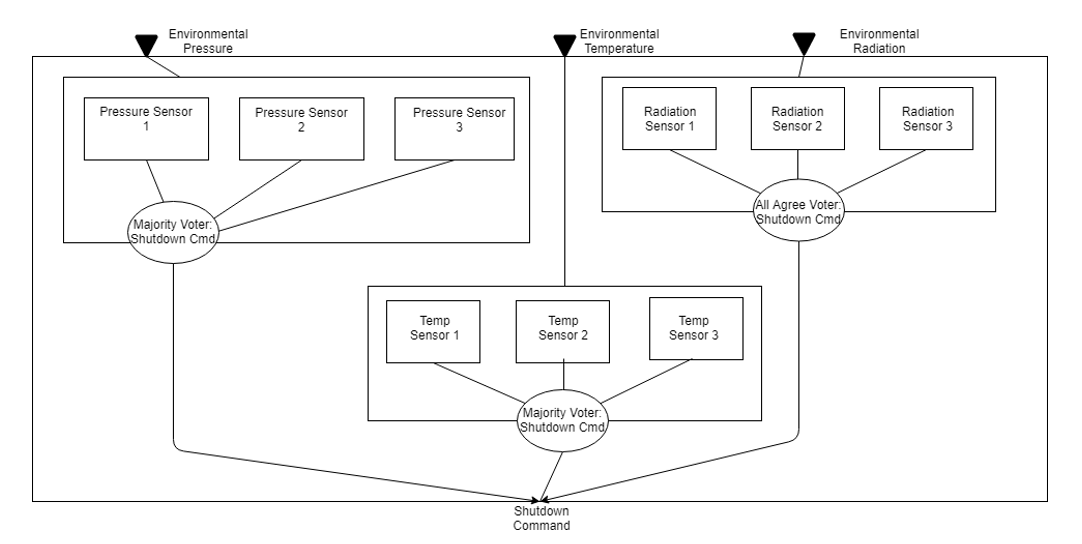
\includegraphics[width=0.6\textwidth]{images/sensorSys.PNG}
	\end{center}
	\vspace{-1em}
	\caption{Pressurized Water Reactor Sensor System}
	\label{fig:sensorSys}
	%\vspace{-2em}
\end{figure*}

\subsection{PWR Nominal Model}
The ``top-level" system is an abstraction of the PWR and contains sensor subsystems. The subsystems contain sensors that monitor pressure, temperature, and radiation. Environmental inputs are fed into each sensor in the model and the redundant sensors monitor temperature, pressure, or radiation respectively. If temperature, pressure, or radiation is too high, a shut down command is sent from the sensors to the parent components. 

The temperature, pressure, and radiation sensor subsystems use a voting mechanism on the redundant sensor values and will send a shut down command based on this output. The safety property of interest in this system is: \emph{shut down when and only when we should}; the AGREE guarantee stating this property is shown in Figure~\ref{fig:shutdownGuar}. 

\begin{figure*}[h!]
	%\vspace{-2em}
	\begin{center}
		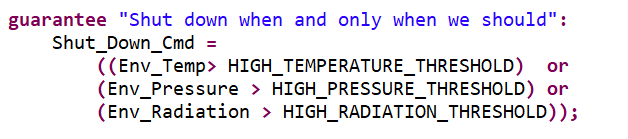
\includegraphics[width=0.5\textwidth]{images/sensorGuar.PNG}
	\end{center}
	\vspace{-2em}
	\caption{Sensor System Safety Property}
	\label{fig:shutdownGuar}
	%\vspace{-2em}
\end{figure*}

The safety of the system requires a shut down to take place if the temperature, pressure, or radiation levels become unsafe; thus, a threshold is introduced and if any sensor subsystem reports passing that threshold, a shutdown command is sent. But on the other hand, we do not want to shut down the system if it is not necessary. If a sensor reports high temperature erroneously and a shut down occurs, this costs time and money. 

Supporting guarantees are located in each sensor subsystem and correspond to temperature, pressure, and radiation sending a shut down command if sensed inputs are above a given threshold. Each sensor has a similar guarantee. 

\subsection{PWR Fault Model}
The faults that are of interest in this example system are any one of the sensors failing high or low. If sensors report high and a shut down command is sent, we shut down when we should not. On the other hand, if sensors report low when it should be high, a shut down command is not sent and we do not shut down when we should. For the remainder of this example, we focus on the failures when sensors report low when they should not.

Two faults are defined with the safety annex for each sensor in the system. An example of a temperature sensor fault stuck at high is shown in Figure~\ref{fig:tempSensorFault}.

\begin{figure*}[h!]
	\vspace{-2em}
	\begin{center}
		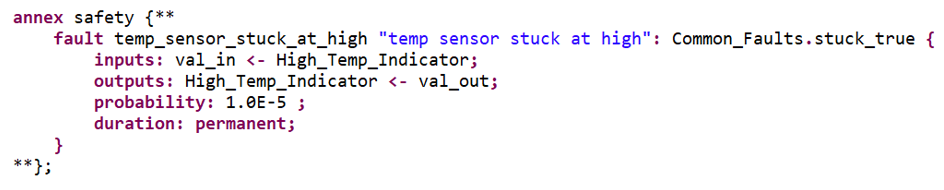
\includegraphics[width=0.8\textwidth]{images/tempSensorFault.PNG}
	\end{center}
	\vspace{-2em}
	\caption{Fault on Temperature Sensor Defined in the Safety Annex for AADL}
	\label{fig:tempSensorFault}
	\vspace{-2em}
\end{figure*}

The Safety Annex provides a way to weave the faults into the nominal model by use of the \emph{inputs} and \emph{outputs} keywords. This allows users to define a fault and attach it to the output of a component. If the fault is active, the error can then in essence violate the guarantees of this component and possibly the assumptions of downstream components~\cite{stewart2020safety}. The activation of a fault is not up to the user, but instead left up to the backend model checker, JKind, to determine if the activation of this fault will contribute to a violation of higher level guarantees. If so, it can be activated during the analysis.

For simplicity, throughout this paper we refer only to faults that fail low (i.e., the environmental input is actually high which warrants a shut down command, but the sensor reports that it is within safe ranges). This simplification is presented to keep the example and results described concise. For ease of reference, a table is provided giving model elements of interest in the sensor example. We refer to these throughout this section. Note: the thresholds vary for pressure, temperature, and radiation. These are given as constants $T_p$, $T_t$, and $T_r$ respectively. The shutdown command is defined notationally as $S$.  The faults are shown as ``fail low" which correspond to the temp (or pressure or radiation) being high, but the sensor reports safe ranges. We also do not list all guarantees and assumptions that are in the model, but only the ones of interest for this analysis. \danielle{Still messing around with how to display this in a way that it isn't messy, doesn't take up a ton of space, and am not currently happy with this approach. But I really hated the tables. Too much info for what is actually needed. Will keep working on this.}

\begin{description}[parsep=0.3ex]
 \item[PWR System:] $P = ((temp$ $>$ $T_t)$ $\lor$ $ (pressure$ $>$ $ T_p)$  $\lor$ $ (radiation$ $>$ $ T_r)) \iff S$\\
 \item[Temp Subsystem]: $G_t = temp$ $>$ $ T_t \iff S$\\
 \item[Pressure Subsystem:] $G_p = pressure$ $>$ $ T_p \iff S$\\
 \item[Radiation Subsystem:] $G_r = radiation$ $>$ $ T_r \iff S$\\
 \item[Temp Sensors (3):] $g_p = pressure$ $>$ $ T_p \iff S$, Fault $f_{ti}$: fails low for $i = 1, 2, 3$.\\
\item[Pressure Sensors (3):] $g_r = radiation$ $>$ $ T_r \iff S$, Fault $f_{pi}$: fails low for $i = 1, 2, 3$. \\
 \item[Radiation Sensors (3):] $g_r = radiation$ $>$ $ T_r \iff S$, Fault $f_{ri}$: fails low for $i = 1, 2, 3$\\
 \end{description}


\begin{comment}
\begin{center}
\resizebox{0.5\textwidth}{!}{%
    \begin{tabular}{ | c | c | c |}
      \hline
      \thead{Component} & \thead{Layer of Analysis} & \thead{Guarantee}\\
      \hline
      ReactorSys & Top &  \makecell{Safety Property $P$: \\ $((temp$ $>$ $T_t)$ $\lor$ $ (pressure$ $>$ $ T_p)$  $\lor$ $ (radiation$ $>$ $ T_r))$ \\ $\iff SHUTDOWN$}    \\
      \hline
      TempSys & Leaf  &  \makecell{Guarantee $G_t$: \\  $temp$ $>$ $ T_t \iff SHUTDOWN$}   \\
      \hline
      PressureSys & Leaf  &  \makecell{Guarantee $G_p$: \\ $pressure$ $>$ $ T_p \iff SHUTDOWN$}    \\
	\hline
      RadiationSys & Leaf  &  \makecell{Guarantee $G_r$: \\ $radiation$ $>$ $ T_r \iff SHUTDOWN$}   \\
      \hline
    \end{tabular}}
  \end{center}

\begin{center}
\resizebox{0.5\textwidth}{!}{%
    \begin{tabular}{ | c | c | c |}
      \hline
      \thead{Component} & \thead{Layer of Architecture} & \thead{Faults}\\
      \hline
      Temp Sensors (3) & \makecell{Leaf \\ Components} & \makecell{$f_{t}$: fail low}  \\
      \hline
	Pressure Sensors (3) & \makecell{Leaf \\ Components} & \makecell{$f_{p}$: fail low}  \\
      \hline
	Radiation Sensors (3) & \makecell{Leaf \\ Components} & \makecell{$f_{r}$: fail low}  \\
      \hline
    \end{tabular}}
  \end{center}



\subsection{Using this Example in the Generation of Minimal Cut Sets}
Step by step, we outline how minimal cut sets are generated through the \aivcalg algorithm using the sensor system as an example. For ease of reference, a table is provided giving model elements of interest in the sensor example. We refer to these throughout this section. Note: the thresholds vary for pressure, temperature, and radiation. These are given as constants $T_p$, $T_t$, and $T_r$ respectively. We also do not list all guarantees and assumptions that are in the model, but only the ones of interest for this analysis.

\begin{center}
\resizebox{\textwidth}{!}{%
    \begin{tabular}{ | c | c | c |}
      \hline
      \thead{Component} & \thead{Layer of Analysis} & \thead{Guarantee}\\
      \hline
      ReactorSys & Top &  \makecell{Safety Property $P$: \\ $((temp$ $>$ $T_t)$ $\lor$ $ (pressure$ $>$ $ T_p)$  $\lor$ $ (radiation$ $>$ $ T_r))$ \\ $\iff SHUTDOWN$}    \\
      \hline
      TempSys & Leaf  &  \makecell{Guarantee $g_t$: \\  $temp$ $>$ $ T_t \iff SHUTDOWN$}   \\
      \hline
      PressureSys & Leaf  &  \makecell{Guarantee $g_p$: \\ $pressure$ $>$ $ T_p \iff SHUTDOWN$}    \\
	\hline
      RadiationSys & Leaf  &  \makecell{Guarantee $g_r$: \\ $radiation$ $>$ $ T_r \iff SHUTDOWN$}   \\
      \hline
    \end{tabular}}
  \end{center}

\begin{center}
%\resizebox{\textwidth}{!}{%
    \begin{tabular}{ | c | c | c |}
      \hline
      \thead{Component} & \thead{Layer of Architecture} & \thead{Faults}\\
      \hline
      Temp Sensors (3) & \makecell{Leaf \\ Components} & \makecell{$f_{t}$: fail low}  \\
      \hline
	Pressure Sensors (3) & \makecell{Leaf \\ Components} & \makecell{$f_{p}$: fail low}  \\
      \hline
	Radiation Sensors (3) & \makecell{Leaf \\ Components} & \makecell{$f_{r}$: fail low}  \\
      \hline
    \end{tabular}
  \end{center}

The first two steps of this process are performed top down in conjunction with JKind analysis over a program. Thus, the top layer is analyzed first, then the next and so on. Steps 3 and 4 proceed after all MIVCs for each layer have been generated. We walk through this sensor system example in this fashion. 

\textbf{Step 1a: Preprocessing top layer.} The preprocessing step inserts specific MIVC elements into the Lustre program. The MIVC elements are the model elements considered in the constraint system for a given property. The Safety Annex provides the means to define a fault over the output of a component. This fault is given an unassigned \emph{trigger} Boolean literal in Lustre. If the trigger literal is true, the output of the component is changed. If not, the output remains equivalent to the nominal output of this component~\cite{stewart2020safety, Stewart17:IMBSA}. This trigger in Lustre is called a \emph{fault activation literal}. The IVC elements required in order to perform this transformation are these fault activation literals as well as guarantees. The basic rules used to insert these additional literals into Lustre depend on the analysis layer of that is being formed in Lustre and are as follows. 
\begin{itemize}
\item Leaf layer of analysis: only fault activation literals are added.
\item Middle or top layers: guarantees are added and if a direct subcomponent is a leaf component of the architecture and faults are defined on its outputs, then these faults are also added.
\end{itemize}

At the top level, guarantees of the sensor subsystems are the IVC elements.
$$\boxed{g_t, g_p, g_r}$$

There are distinct constraint systems, one for each property being proved. In this system at the top layer, there is a single property $P$; this results in the following constraint system. 
$$\boxed{C = \{g_t, g_p, g_r, \neg P\}}$$

\textbf{Step 2a: Generate all MIVCs for the constraint system at the top layer.} In order to prove $P$, all three guarantees from the sensor subsystem level are required. 
$$\boxed{MIVC(P) = \{g_t, g_p, g_r\}}$$. 

\textbf{Step 1b: Preprocessing leaf layer.} Model elements for the IVC algorithm consideration are the faults for each sensor, for instance temperature sensors:
$$\boxed{f_{t1}, f_{t2}, f_{t3}}$$ 

The resulting constraint system for the temperature sensor subsystem layer is:
$$\boxed{C = \{\neg f_{t1}, \neg f_{t2}, \neg f_{t3}, \neg g_t\}}$$

\textbf{Step 2b: Generate all MIVCs for the constraint system at the leaf layer.} Due to the majority voting mechanism, the MIVCs show all possible pairs of faults restricted to \emph{false}. This means, if any combination of two faults do not occur, then the guarantees at the temperature sensor subsystem level are satisfied. 
$$\boxed{
	\begin{aligned}
		MIVC_1(g_t) = \{\neg f_{t1}, \neg f_{t2}\} \\
		MIVC_2(g_t) = \{\neg f_{t1}, \neg f_{t3}\} \\
		MIVC_3(g_t) = \{\neg f_{t2}, \neg f_{t3}\}
	\end{aligned}
}$$

At this point, all MIVCs have been successfully generated (which is a requirement of the following algorithms) and we can move on to the generation of minimal cut sets. 

\textbf{Step 3a: Generate MCSs using a hitting set algorithm at the top layer.} Our single MIVC in this case will reveal three associated MCSs. (Notice: $MCS_1 \cap MIVC(P) \neq \emptyset$, and same for $MCS_2$ and $MCS_3$, thus these are hitting sets.)
 $$\boxed{
	\begin{aligned}
		MCS_1(top) = \{g_t\} \\
		MCS_2(top) = \{g_p\} \\
		MCS_3(top) = \{g_r\}
	\end{aligned}
}$$

\textbf{Step 4a: Transform MCSs into MinCutSets at the top layer.} Given that only guarantees are found in the MCSs at this layer, recursion is used to find the faults that cause violation of these guarantees. Using this recursion on $MCS_1$, we show the process further. 

\textbf{Step 3b: Generate MCSs using a hitting set algorithm at the leaf layer.} In step 2b, we found all MIVCs for the contract $g_t$ and send these to the hitting set algorithm. The resulting MCSs are: 
 $$\boxed{
	\begin{aligned}
		MCS_1(leaf) = \{\neg f_{t1}, \neg f_{t2}\} \\
		MCS_2(leaf) = \{\neg f_{t1}, \neg f_{t3}\} \\
		MCS_3(leaf) = \{\neg f_{t2}, \neg f_{t3}\}
	\end{aligned}
}$$

Only constrained faults are found in these MCSs, so we simply remove those constraints and have found the MinCutSets for the contracts $g_t$. These are returned and replace this contract in the top layer $MCS_1(top)$. Here is the end result for $MCS_1(top)$; this can be understood as three of the total minimal cut sets for $P$. 

\begin{equation*}
MCS_1(top) \rightarrow \left\{ \,
\begin{IEEEeqnarraybox}[][c]{l?s}
\IEEEstrut
MinCutSet_1(P) = \{f_{t1}, f_{t2}\}, \\
MinCutSet_2(P) = \{f_{t1},  f_{t3}\}, \\
MinCutSet_3(P) = \{f_{t2}, f_{t3}\}
\IEEEstrut
\end{IEEEeqnarraybox}
\right.
\end{equation*}

After all replacements have been made, we are left with all minimal cut sets for the property of interest ($P$ in this example). 

\end{comment}











%\section{Preliminaries}
\label{sec:background}
One of our goals is to transition the tools we have developed into use by the safety engineers who perform safety assessment of avionics products. Therefore, we need to understand how the tools and the models will fit into the existing safety assessment and certification process. Part of this understanding involves taking a look at pertinent background information in safety analysis. 

\subsection{Safety Critical Systems}
\label{sec:SA_background}
A safety critical system is a system whose safety cannot be shown solely by test, whose logic is difficult to comprehend without the aid of analytical tools, and whose failure can directly or indirectly cause significant loss of life or property\cite{SAE:ARP4761}. Guaranteeing safety and reliability of safety critical systems is mandatory. The process that guides this guarantee is highly standardized and controlled~\cite{RTCA:StdC,SAE:ARP4761} . Due to the complexity of critical systems, the field of safety analysis has in recent decades turned to formal methods~\cite{mattarei,Bozzano:2010:DSA:1951720}. In practice, a systems behavior can be described in a variety of ways that include diagrams, textual descriptions, and operational procedures~\cite{SAE:ARP4754A}. These descriptions must be clear and well defined in order to avoid ambiguous interpretation. The formal definition of system behavior has a unique interpretation and is therefore a good candidate for automated analysis in order to validate requirements and spot design flaws~\cite{Joshi05:Dasc}. 

Model checking is a technique used to allow exhaustive and automatic checking of whether a system model (formal system definition) meets a set of formal requirements. As early as the '90's, using model checking for safety requirements began to surface in the critical systems literature\cite{DBLP:conf/safecomp/CimattiGMRTT98,DBLP:conf/edcc/BernardeschiFGM96}. Current tools in safety analysis use model checking techniques during the development and assessment of safety critical systems, \cite{mattarei,CAV2015:BoCiGrMa,symbAltaRica,DBLP:conf/tacas/BittnerBCCGGMMZ16}.







\subsection{Model Based Safety Analysis}
\label{sec:mbsa}

Safety engineers traditionally perform safety analysis based on information synthesized from a variety of sources including informal design models and requirement documents. These analyses are highly subjective and dependent on the skill of the analyst. The lack of precise models requires the analyst to devote a fair amount of time to information gathering of the architecture and behavior of the system. On the other hand, in Model Based Safety Aanalysis (MBSA), the system and safety engineers share a common system model created using the model based development process. By extending the system model and relevant physical control systems, automated support can be provided for much of the safety analysis. Using a common model for both system and safety engineering and automating parts of safety analysis assists in the reduction of cost and improves the quality of the safety analysis, but this is not without disadvantages if the model itself is faulty. 

In model based system development, various development activities such as simulation, verification, testing, and code generation are based on a formal model of the system under development\cite{Joshi05:Dasc}. This is called the nominal model. Model based development was extended to include model based safety analysis\cite{Joshi05:Dasc,Joshi05:SafeComp,Joshi07:Hase,DBLP:conf/cav/BozzanoCPJKPRT15,CAV2015:BoCiGrMa,info17:HaLuHo}. The goal of MBSA is to incorporate safety analysis into the model based development process in order to provide information on the safety of the formal model of the system under development. In this process, the nominal (non-failure) system behavior that is captured in the model based development process is augmented with the fault behavior of the system. Model based safety analysis then operates on a formal model that describes both nominal system behavior and the fault model, which describes fault behavior. 






\subsection{Safety Assessment Process}
\label{subsec:process}

ARP4761, the Guidelines and Methods for Conducting Safety Assessment Process on Civil Airborne Systems and Equipment, provides guidance on applying development assurance at each hierarchical level throughout the development life cycle of highly-integrated/complex aircraft systems, and has been recognized by the Federal Aviation Administration (FAA) as an acceptable method to establish the assurance process~\cite{SAE:ARP4761}.

\begin{figure*}[h!]
	%\vspace{-0.956in}
	\centering
	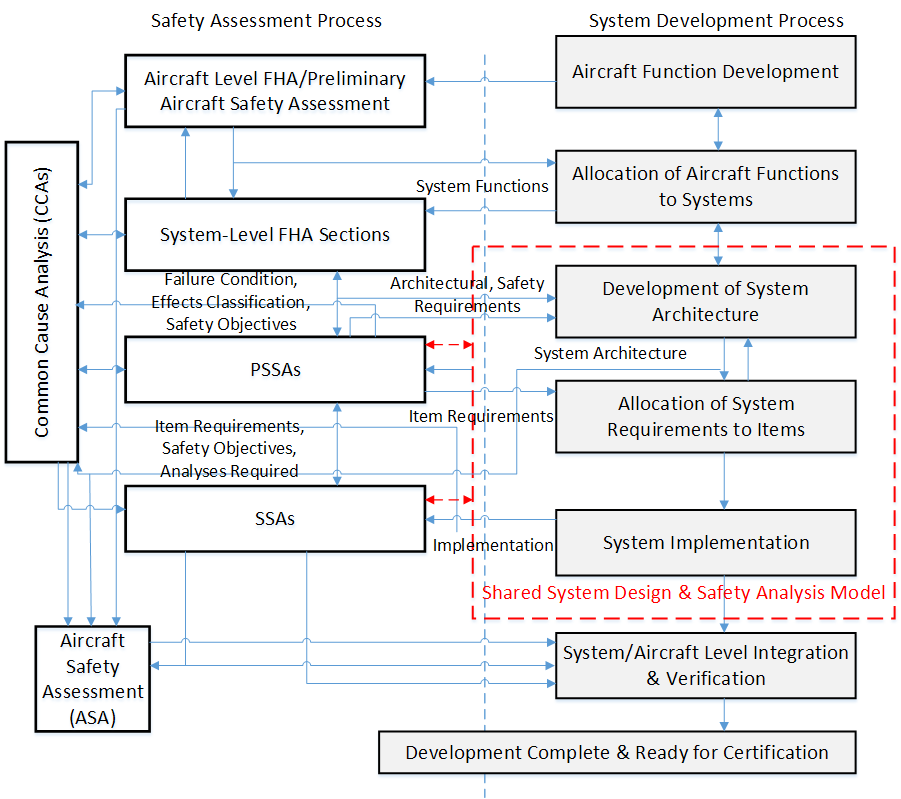
\includegraphics[width=1.0\textwidth]{images/Safety_Assessment_Process.png}
	%\vspace{-0.4in}
	\caption{Using the Shared System/Safety Model in the ARP4754A Safety Assessment Process}
	\label{fig:proposed_safety_process}
\end{figure*}

The safety assessment process is part of the development life cycle, and is tightly coupled with the system development and verification processes. It is used to show compliance with certification requirements and for meeting a company's internal safety standards. The guidelines presented in ARP4761 include various industry accepted safety assessment practices. They are summarized here for convenience. 

\begin{itemize}
\item Functional Hazard Assessment (FHA): This process examines aircraft and system functions to identify potential functional failures and classifies the hazards associated with specific failure conditions. This is usually developed early in the development process and is updated throughout. 

\item Preliminary System Safety Assessment (PSSA): This will establish the system safety requirements and provide some indication that the system architecture can meet those safety requirements. This is also updated throughout the development process.

\item System Safety Assessment (SSA): This process collects, analyzes, and documents verification that the system, as implemented, meets the safety requirements established by the PSSA. 

\item Common Cause Analysis (CCA): The CCA establishes physical and functional separation, isolation, and independence requirements between systems and verifies that these requirements have been met.
\end{itemize}

As shown in Figure~\ref{fig:proposed_safety_process}, these processes occur during the development process and are continually updated throughout. The safety engineers then use the acquired understanding to conduct safety analysis, construct the safety analysis artifacts, and compare the analysis results with established safety objectives and safety-related requirements. 

In practice, prior to performing the safety assessment of a system, the safety engineers are often equipped with the domain knowledge about the system, but do not necessarily have detailed knowledge of how the software functions are designed. Acquiring the required knowledge about the behavior and implementation of each software function in a system can be time-consuming. Industry practitioners have come to realize the benefits and importance of using models to assist the safety assessment process (either by augmenting the existing system design model, or by building a separate safety model), and a revision of the ARP4761 to include model based safety analysis is under way. Capturing failure modes in models and generating safety analysis artifacts directly from models could greatly improve communication and synchronization between system designer and safety engineers, and provide the ability to more accurately analyze complex systems. 

A single unified model to conduct both system development and safety analysis can help reduce the gap in comprehending the system behavior and transferring the knowledge between the system designers and the safety analysts. This maintains a living model that captures the current state of the system design as it moves through the system development lifecycle.

A single unified model also allows all participants of the ARP4754A process to be able to communicate and review the system design using a ``single source of truth.''

A model that supports both system design and safety analysis must describe both the system design information (e.g., system architecture, functional behavior) and safety-relevant information (e.g., failure modes, failure rates).  It must do this in a way that keeps the two types of information distinguishable, yet allows them to interact with each other.

Figure~\ref{fig:proposed_safety_process} presents our proposed use of this shared system design and safety analysis model in the context of the ARP4754A Safety Assessment Process Model (derived from Figure 7 of ARP4754A). The shared model is one of the system development artifacts from the ``Development of System Architecture'' and ``Allocation of System Requirements to Item'' activities in the System Development Process, which interacts with the PSSAs and SSAs activities in the Safety Assessment Process. This is seen as a box labeled ``Shared System Design and Safety model'' on the right column of the figure. The shared model can serve as an interface to capture the information from the system design and implementation that is relevant for the safety analysis.






%\section{Running Example}
\label{sec:example}

To illustrate the generation of minimal cut sets through the use of IVCs, we present a running example of a sensor system in a Pressurized Water Reactor (PWR). In a typical PWR, the core inside of the reactor vessel produces heat. Pressurized water in the primary coolant loop carries the heat to the steam generator. Within the steam generator, heat from the primary coolant loop vaporizes the water in a secondary loop, producing steam. The steamline directs the steam to the main turbine, causing it to turn the turbine generator, which produces electricity. There are a few important factors that must be considered during safety assessment and system design. An unsafe climb in temperature can cause high pressure and hence pipe rupture, and high levels of radiation could indicate a leak of primary coolant. The following sensor system can be thought of as a subsystem within a PWR that monitors these factors. A diagram of the AADL model is shown in Figure~\ref{fig:sensorSys} and represents a highly simplified version of a safety critical system. \danielle{May add cartoon figure demonstrating this model/process later - depending on space. Also can adjust figure placement after rewriting, adding, and cutting is done.}

\begin{figure*}[h!]
	%\vspace{-2em}
	\begin{center}
		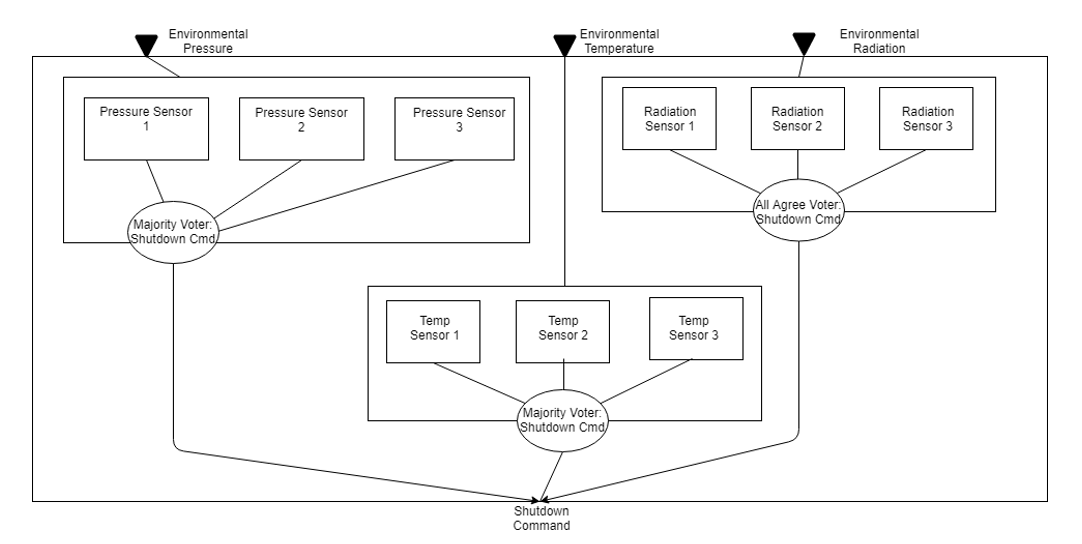
\includegraphics[width=0.6\textwidth]{images/sensorSys.PNG}
	\end{center}
	\vspace{-1em}
	\caption{Pressurized Water Reactor Sensor System}
	\label{fig:sensorSys}
	%\vspace{-2em}
\end{figure*}

\subsection{PWR Nominal Model}
The ``top-level" system is an abstraction of the PWR and contains sensor subsystems. The subsystems contain sensors that monitor pressure, temperature, and radiation. Environmental inputs are fed into each sensor in the model and the redundant sensors monitor temperature, pressure, or radiation respectively. If temperature, pressure, or radiation is too high, a shut down command is sent from the sensors to the parent components. 

The temperature, pressure, and radiation sensor subsystems use a voting mechanism on the redundant sensor values and will send a shut down command based on this output. The safety property of interest in this system is: \emph{shut down when and only when we should}; the AGREE guarantee stating this property is shown in Figure~\ref{fig:shutdownGuar}. 

\begin{figure*}[h!]
	%\vspace{-2em}
	\begin{center}
		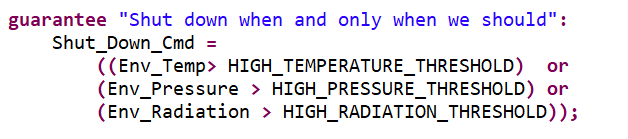
\includegraphics[width=0.5\textwidth]{images/sensorGuar.PNG}
	\end{center}
	\vspace{-2em}
	\caption{Sensor System Safety Property}
	\label{fig:shutdownGuar}
	%\vspace{-2em}
\end{figure*}

The safety of the system requires a shut down to take place if the temperature, pressure, or radiation levels become unsafe; thus, a threshold is introduced and if any sensor subsystem reports passing that threshold, a shutdown command is sent. But on the other hand, we do not want to shut down the system if it is not necessary. If a sensor reports high temperature erroneously and a shut down occurs, this costs time and money. 

Supporting guarantees are located in each sensor subsystem and correspond to temperature, pressure, and radiation sending a shut down command if sensed inputs are above a given threshold. Each sensor has a similar guarantee. 

\subsection{PWR Fault Model}
The faults that are of interest in this example system are any one of the sensors failing high or low. If sensors report high and a shut down command is sent, we shut down when we should not. On the other hand, if sensors report low when it should be high, a shut down command is not sent and we do not shut down when we should. For the remainder of this example, we focus on the failures when sensors report low when they should not.

Two faults are defined with the safety annex for each sensor in the system. An example of a temperature sensor fault stuck at high is shown in Figure~\ref{fig:tempSensorFault}.

\begin{figure*}[h!]
	\vspace{-2em}
	\begin{center}
		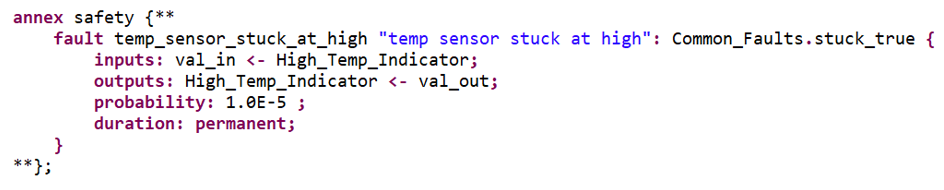
\includegraphics[width=0.8\textwidth]{images/tempSensorFault.PNG}
	\end{center}
	\vspace{-2em}
	\caption{Fault on Temperature Sensor Defined in the Safety Annex for AADL}
	\label{fig:tempSensorFault}
	\vspace{-2em}
\end{figure*}

The Safety Annex provides a way to weave the faults into the nominal model by use of the \emph{inputs} and \emph{outputs} keywords. This allows users to define a fault and attach it to the output of a component. If the fault is active, the error can then in essence violate the guarantees of this component and possibly the assumptions of downstream components~\cite{stewart2020safety}. The activation of a fault is not up to the user, but instead left up to the backend model checker, JKind, to determine if the activation of this fault will contribute to a violation of higher level guarantees. If so, it can be activated during the analysis.

For simplicity, throughout this paper we refer only to faults that fail low (i.e., the environmental input is actually high which warrants a shut down command, but the sensor reports that it is within safe ranges). This simplification is presented to keep the example and results described concise. For ease of reference, a table is provided giving model elements of interest in the sensor example. We refer to these throughout this section. Note: the thresholds vary for pressure, temperature, and radiation. These are given as constants $T_p$, $T_t$, and $T_r$ respectively. The shutdown command is defined notationally as $S$.  The faults are shown as ``fail low" which correspond to the temp (or pressure or radiation) being high, but the sensor reports safe ranges. We also do not list all guarantees and assumptions that are in the model, but only the ones of interest for this analysis. \danielle{Still messing around with how to display this in a way that it isn't messy, doesn't take up a ton of space, and am not currently happy with this approach. But I really hated the tables. Too much info for what is actually needed. Will keep working on this.}

\begin{description}[parsep=0.3ex]
 \item[PWR System:] $P = ((temp$ $>$ $T_t)$ $\lor$ $ (pressure$ $>$ $ T_p)$  $\lor$ $ (radiation$ $>$ $ T_r)) \iff S$\\
 \item[Temp Subsystem]: $G_t = temp$ $>$ $ T_t \iff S$\\
 \item[Pressure Subsystem:] $G_p = pressure$ $>$ $ T_p \iff S$\\
 \item[Radiation Subsystem:] $G_r = radiation$ $>$ $ T_r \iff S$\\
 \item[Temp Sensors (3):] $g_p = pressure$ $>$ $ T_p \iff S$, Fault $f_{ti}$: fails low for $i = 1, 2, 3$.\\
\item[Pressure Sensors (3):] $g_r = radiation$ $>$ $ T_r \iff S$, Fault $f_{pi}$: fails low for $i = 1, 2, 3$. \\
 \item[Radiation Sensors (3):] $g_r = radiation$ $>$ $ T_r \iff S$, Fault $f_{ri}$: fails low for $i = 1, 2, 3$\\
 \end{description}


\begin{comment}
\begin{center}
\resizebox{0.5\textwidth}{!}{%
    \begin{tabular}{ | c | c | c |}
      \hline
      \thead{Component} & \thead{Layer of Analysis} & \thead{Guarantee}\\
      \hline
      ReactorSys & Top &  \makecell{Safety Property $P$: \\ $((temp$ $>$ $T_t)$ $\lor$ $ (pressure$ $>$ $ T_p)$  $\lor$ $ (radiation$ $>$ $ T_r))$ \\ $\iff SHUTDOWN$}    \\
      \hline
      TempSys & Leaf  &  \makecell{Guarantee $G_t$: \\  $temp$ $>$ $ T_t \iff SHUTDOWN$}   \\
      \hline
      PressureSys & Leaf  &  \makecell{Guarantee $G_p$: \\ $pressure$ $>$ $ T_p \iff SHUTDOWN$}    \\
	\hline
      RadiationSys & Leaf  &  \makecell{Guarantee $G_r$: \\ $radiation$ $>$ $ T_r \iff SHUTDOWN$}   \\
      \hline
    \end{tabular}}
  \end{center}

\begin{center}
\resizebox{0.5\textwidth}{!}{%
    \begin{tabular}{ | c | c | c |}
      \hline
      \thead{Component} & \thead{Layer of Architecture} & \thead{Faults}\\
      \hline
      Temp Sensors (3) & \makecell{Leaf \\ Components} & \makecell{$f_{t}$: fail low}  \\
      \hline
	Pressure Sensors (3) & \makecell{Leaf \\ Components} & \makecell{$f_{p}$: fail low}  \\
      \hline
	Radiation Sensors (3) & \makecell{Leaf \\ Components} & \makecell{$f_{r}$: fail low}  \\
      \hline
    \end{tabular}}
  \end{center}



\subsection{Using this Example in the Generation of Minimal Cut Sets}
Step by step, we outline how minimal cut sets are generated through the \aivcalg algorithm using the sensor system as an example. For ease of reference, a table is provided giving model elements of interest in the sensor example. We refer to these throughout this section. Note: the thresholds vary for pressure, temperature, and radiation. These are given as constants $T_p$, $T_t$, and $T_r$ respectively. We also do not list all guarantees and assumptions that are in the model, but only the ones of interest for this analysis.

\begin{center}
\resizebox{\textwidth}{!}{%
    \begin{tabular}{ | c | c | c |}
      \hline
      \thead{Component} & \thead{Layer of Analysis} & \thead{Guarantee}\\
      \hline
      ReactorSys & Top &  \makecell{Safety Property $P$: \\ $((temp$ $>$ $T_t)$ $\lor$ $ (pressure$ $>$ $ T_p)$  $\lor$ $ (radiation$ $>$ $ T_r))$ \\ $\iff SHUTDOWN$}    \\
      \hline
      TempSys & Leaf  &  \makecell{Guarantee $g_t$: \\  $temp$ $>$ $ T_t \iff SHUTDOWN$}   \\
      \hline
      PressureSys & Leaf  &  \makecell{Guarantee $g_p$: \\ $pressure$ $>$ $ T_p \iff SHUTDOWN$}    \\
	\hline
      RadiationSys & Leaf  &  \makecell{Guarantee $g_r$: \\ $radiation$ $>$ $ T_r \iff SHUTDOWN$}   \\
      \hline
    \end{tabular}}
  \end{center}

\begin{center}
%\resizebox{\textwidth}{!}{%
    \begin{tabular}{ | c | c | c |}
      \hline
      \thead{Component} & \thead{Layer of Architecture} & \thead{Faults}\\
      \hline
      Temp Sensors (3) & \makecell{Leaf \\ Components} & \makecell{$f_{t}$: fail low}  \\
      \hline
	Pressure Sensors (3) & \makecell{Leaf \\ Components} & \makecell{$f_{p}$: fail low}  \\
      \hline
	Radiation Sensors (3) & \makecell{Leaf \\ Components} & \makecell{$f_{r}$: fail low}  \\
      \hline
    \end{tabular}
  \end{center}

The first two steps of this process are performed top down in conjunction with JKind analysis over a program. Thus, the top layer is analyzed first, then the next and so on. Steps 3 and 4 proceed after all MIVCs for each layer have been generated. We walk through this sensor system example in this fashion. 

\textbf{Step 1a: Preprocessing top layer.} The preprocessing step inserts specific MIVC elements into the Lustre program. The MIVC elements are the model elements considered in the constraint system for a given property. The Safety Annex provides the means to define a fault over the output of a component. This fault is given an unassigned \emph{trigger} Boolean literal in Lustre. If the trigger literal is true, the output of the component is changed. If not, the output remains equivalent to the nominal output of this component~\cite{stewart2020safety, Stewart17:IMBSA}. This trigger in Lustre is called a \emph{fault activation literal}. The IVC elements required in order to perform this transformation are these fault activation literals as well as guarantees. The basic rules used to insert these additional literals into Lustre depend on the analysis layer of that is being formed in Lustre and are as follows. 
\begin{itemize}
\item Leaf layer of analysis: only fault activation literals are added.
\item Middle or top layers: guarantees are added and if a direct subcomponent is a leaf component of the architecture and faults are defined on its outputs, then these faults are also added.
\end{itemize}

At the top level, guarantees of the sensor subsystems are the IVC elements.
$$\boxed{g_t, g_p, g_r}$$

There are distinct constraint systems, one for each property being proved. In this system at the top layer, there is a single property $P$; this results in the following constraint system. 
$$\boxed{C = \{g_t, g_p, g_r, \neg P\}}$$

\textbf{Step 2a: Generate all MIVCs for the constraint system at the top layer.} In order to prove $P$, all three guarantees from the sensor subsystem level are required. 
$$\boxed{MIVC(P) = \{g_t, g_p, g_r\}}$$. 

\textbf{Step 1b: Preprocessing leaf layer.} Model elements for the IVC algorithm consideration are the faults for each sensor, for instance temperature sensors:
$$\boxed{f_{t1}, f_{t2}, f_{t3}}$$ 

The resulting constraint system for the temperature sensor subsystem layer is:
$$\boxed{C = \{\neg f_{t1}, \neg f_{t2}, \neg f_{t3}, \neg g_t\}}$$

\textbf{Step 2b: Generate all MIVCs for the constraint system at the leaf layer.} Due to the majority voting mechanism, the MIVCs show all possible pairs of faults restricted to \emph{false}. This means, if any combination of two faults do not occur, then the guarantees at the temperature sensor subsystem level are satisfied. 
$$\boxed{
	\begin{aligned}
		MIVC_1(g_t) = \{\neg f_{t1}, \neg f_{t2}\} \\
		MIVC_2(g_t) = \{\neg f_{t1}, \neg f_{t3}\} \\
		MIVC_3(g_t) = \{\neg f_{t2}, \neg f_{t3}\}
	\end{aligned}
}$$

At this point, all MIVCs have been successfully generated (which is a requirement of the following algorithms) and we can move on to the generation of minimal cut sets. 

\textbf{Step 3a: Generate MCSs using a hitting set algorithm at the top layer.} Our single MIVC in this case will reveal three associated MCSs. (Notice: $MCS_1 \cap MIVC(P) \neq \emptyset$, and same for $MCS_2$ and $MCS_3$, thus these are hitting sets.)
 $$\boxed{
	\begin{aligned}
		MCS_1(top) = \{g_t\} \\
		MCS_2(top) = \{g_p\} \\
		MCS_3(top) = \{g_r\}
	\end{aligned}
}$$

\textbf{Step 4a: Transform MCSs into MinCutSets at the top layer.} Given that only guarantees are found in the MCSs at this layer, recursion is used to find the faults that cause violation of these guarantees. Using this recursion on $MCS_1$, we show the process further. 

\textbf{Step 3b: Generate MCSs using a hitting set algorithm at the leaf layer.} In step 2b, we found all MIVCs for the contract $g_t$ and send these to the hitting set algorithm. The resulting MCSs are: 
 $$\boxed{
	\begin{aligned}
		MCS_1(leaf) = \{\neg f_{t1}, \neg f_{t2}\} \\
		MCS_2(leaf) = \{\neg f_{t1}, \neg f_{t3}\} \\
		MCS_3(leaf) = \{\neg f_{t2}, \neg f_{t3}\}
	\end{aligned}
}$$

Only constrained faults are found in these MCSs, so we simply remove those constraints and have found the MinCutSets for the contracts $g_t$. These are returned and replace this contract in the top layer $MCS_1(top)$. Here is the end result for $MCS_1(top)$; this can be understood as three of the total minimal cut sets for $P$. 

\begin{equation*}
MCS_1(top) \rightarrow \left\{ \,
\begin{IEEEeqnarraybox}[][c]{l?s}
\IEEEstrut
MinCutSet_1(P) = \{f_{t1}, f_{t2}\}, \\
MinCutSet_2(P) = \{f_{t1},  f_{t3}\}, \\
MinCutSet_3(P) = \{f_{t2}, f_{t3}\}
\IEEEstrut
\end{IEEEeqnarraybox}
\right.
\end{equation*}

After all replacements have been made, we are left with all minimal cut sets for the property of interest ($P$ in this example). 

\end{comment}










%\section{Formalization of the Method}
\label{sec:theory}

\begin{comment}
The main idea that we present in this research is as follows. The MIVCs are MUSs (Minimal Unsatisfiable Subsets) of a constraint system that normally consists of the assumptions and guarantees of system components and the negation of the safety property of interest. The MCSs (Minimal Correction Sets), the sets that contain the minimal ``correction" of the infeasible constraint system, can then be obtained from all MUSs. Here is the key idea that we present: if the constraint system is defined to take into account fault activation literals as well as component contracts, these MCSs and the information they contain can be transformed into MinCutSets. A small example will illustrate this point nicely. 

Let a constraint system $C$ consist of guarantees $g_1$, $g_2$, fault activation literals constrained to $false$, $\neg f_1$, $\neg f_2$, and the safety property $P$ also constrained to $false$, $\neg P$. 
\begin{equation}
    C = \{\neg f_1, \neg f_2, g_1, g_2, \neg P\}
\end{equation}

Now, since we assume that the nominal model proves, it is no surprise that $C$ is UNSAT. (The guarantees are valid, no faults occur, and we want to prove the negation of the safety property.) The MIVC algorithm returns the minimal unsatisfiable subsets, say $MIVC_1 = \{\neg f_1, g_2\}$ and $MIVC_2 = \{\neg f_2\}$. Let us focus on $MIVC_1$. This can be understood in two ways: (1) $MIVC_1$ is a proof core: if $f_1$ does not occur and $g_2$ holds, then the property $P$ can be proven, or (2) $MIVC_1$ is a minimal unsatisfiable subset: it cannot be the case that $f_1$ does not occur and the guarantee $g_2$ holds. 

Next we look at the MCSs for this example:
\begin{center}
    $MCS_1 = \{\neg f_1, \neg f_2\}$,
    $MCS_2 = \{\neg f_2, g_2\}$
\end{center}

This means that $C \setminus MCS_1$ is SAT. So by removing those constraints from $C$, we get a SAT constraint system: $C \setminus MCS_1 = \{f_1, f_2, g_1, g_2, \neg P\}$. When both faults $f_1$ and $f_2$ are active, $\neg P$ can be proven; i.e., this is a cut set for $\neg P$. The minimality of the MCS gives the minimality of the cut set. 
\end{comment}









Throughout the remainder of this section, we provide the formal background necessary to show how this approach works.

In the case of a nominal model augmented with faults, a constraint system can be defined as follows. Let $F$ be the set of all fault activation literals defined in the system and $G$ be the set of component contracts (guarantees of component output behavior). 

\begin{definition}Let $C = \{C_1,C_2,...,C_n\}$ be a constraint system such that for $i \in \{1,...,n\}$, $C_i$ has the following constraints for any $f_j \in F$ and $g_k \in G$ with regard to the top level property $P$: 
\begin{center}
$C_i \in \left\{ \begin{array}{ll}
	f_j :&  false\\
	g_k :& true\\
	P :& false\\
\end{array}\right.$	
\end{center}
\label{def:constraintsystem}
\end{definition}

\begin{comment}
The \aivcalg algorithm collects all minimal unsatisfiable subsets of a given transition system in terms of the \textit{negation} of the top level property~\cite{Ghassabani2017EfficientGO,bendik2018online}. Assuming that the nominal model proves (no faults are active), it is not surprising that the guarantees and the negation of the safety property is UNSAT. The MUSs are the minimal explanation of the infeasibility of this constraint system; equivalently, these are the minimal sets of model elements necessary for proof of the safety property.

We utilize this algorithm by providing not only component contracts as model elements, but also fault activation literals constrained to \textit{false}, i.e., the faults are inactive. Thus the resulting MIVCs (MUSs) will contain the required contracts and constrained fault activation literals necessary to prove the safety property. 

Because of the duality between MUSs and MCSs, all MCSs can be obtained by finding the hitting sets of all MUSs. The MCS can be seen to correct the infeasibility of the constraint system and provides the minimal such correction. By removing the constraints from $C$ that are found in any MCS, $C$ becomes satisfiable. In terms of the constraint system that includes fault activation literals, by \textit{activating} the faults in the MCS and \textit{violating} the contracts in the MCS, we can prove the \textit{negation} of the property $P$. This is the precise information we require to find the minimal cut sets of a system. If the contracts in the MCS are replaced with the faults that cause its violation, the MCS is transformed into a MinCutSet. A high level summary of the steps of this transformation are shown in Figure~\ref{fig:trans}. 

\begin{figure*}[h!]
	%\vspace{-0.1in}
	\begin{center}
		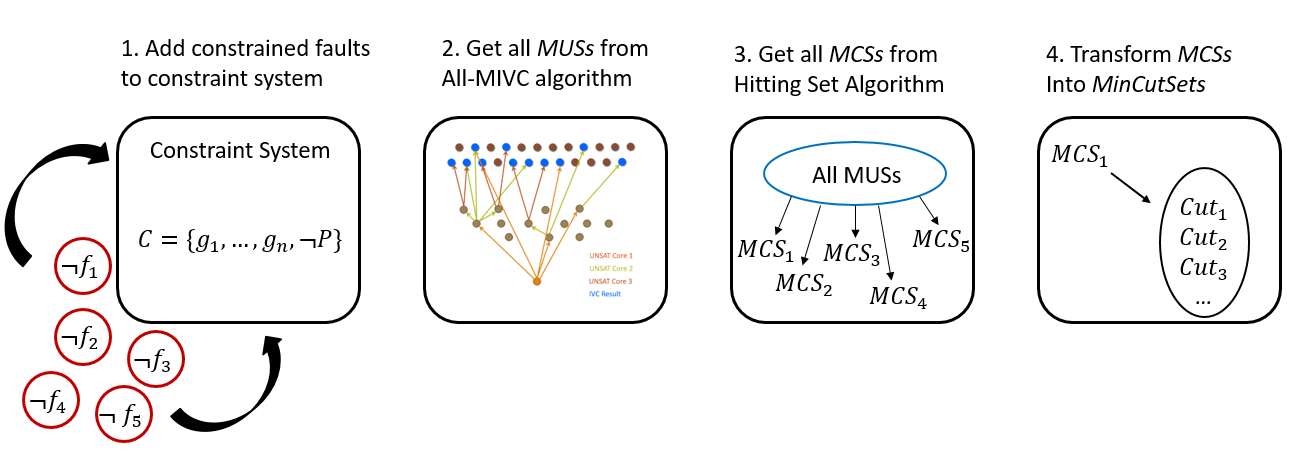
\includegraphics[width=0.8\textwidth]{images/highLevelIdea.PNG}
	\end{center}
	\caption{Steps of the Transformation Process}
	\label{fig:trans}
\end{figure*}

\danielle{End of copy/paste.}

\end{comment}
The theory regarding MIVCs and the duality of MUSs with MCSs has been established~\cite{GhassabaniGW16,Ghassabani2017EfficientGO,liffiton2016fast}. The MCSs are transformed into Minimal Cut Sets according to the following theoretical results. We assume that the nominal model proves a safety property $P$. Then since the nominal model consists of all its component contracts, $G$, and all faults constrained to false, $F$, we can say that $F \cup G$ satisfies $P$ and the constraint system $C = F \cup G \cup \{\neg P\}$ is UNSAT for disjoint sets $F$ and $G$.

Let the set $\overline{MCS}$ be an MCS with all constraints removed.

\begin{lemma}
$\overline{MCS}$ satisfies $\neg P$.

%If the only elements of a MCS are constrained faults, these unconstrained faults are a minimal cut set.
\begin{proof}
Let $\overline{MCS}$ consist of the elements of MCS with constraints removed and let $C = E \cup \{\neg P\}$ for all model elements $E$ (i.e., $E = F \cup G$). Since $C$ is UNSAT, clearly $E$ does not satisfy $\neg P$. \\

Since $MCS \subseteq E$, we can further decompose $E$. Let the set $L_E$ be all elements of $E$ that are not found in $MCS$; the leftover elements. Then $E = L_E \cup MCS$ for disjoint sets $L_E$ and $MCS$. \\

It follows that since $E$ does not satisfy $\neg P$, we know that neither $L_E$ nor $MCS$ satisfies $\neg P$.\\ 

But we also know by the definition of $MCS$ that $C \setminus MCS$ satisfies $\neg P$ (i.e., removing all constraints from the elements in $C$ that are found in the $MCS$ produces a satisfiable constraint system). \\

Let $\overline{MCS}$ be the MCS with all constraints removed. Then $C \setminus MCS$ can be represented as: $C = L_E \cup \overline{MCS} \cup \{\neg P\}$ which is satisfiable. \\

Since $L_E$ does not satisfy $\neg P$, it must be the case that $\overline{MCS}$ does satisfy $\neg P$.

\end{proof}
\label{lem:minCorrSet1}
\end{lemma}
\vspace{-2em}

In order to transform the MCS into a minimal cut set, any contracts found in the MCS must be replaced with faults that cause their violation. We show that making this replacement still satisfies $\neg P$.

\begin{lemma}
	Replacement of a contract $g \in \overline{MCS}$ with the faults that cause its violation satisfies $\neg P$.
	\begin{proof}
	Assume that there exists a $g \in G$ where $g \in MCS$. Given the assumption that $G \cup \{P\}$ is SAT (i.e., the nominal model proves), $\neg g$ can only occur by activation of faults. For the set of all faults in the system, $F$, let $F_G \subseteq F$ such that $F_G$ satisfies $\neg g$ and let $F_G$ be a minimal such set (i.e. $F_G$ is a minimal cut set for $g$). Replace $g \in \overline{MCS}$ with $F_G$; call this new set $MCS_{repl}$. By the assumption that $F_G$ satisfies $\neg g$ and lemma 1, the result is immediate.
	\end{proof}
	\label{lem:corrSet}
\end{lemma}
\vspace{-2em}

\begin{lemma}
$MCS_{repl}$ is minimal.
\begin{proof}
The minimality follows directly from the definition of MCS. 

\end{proof}
\label{lem:minCorrSet}
\end{lemma}
\vspace{-2em}
Once all replacements have been made, the set $MCS_{repl}$ contains only faults. Since $MCS_{repl}$ satisfies $\neg P$, these unconstrained faults are a cut set for $\neg P$. Thus, iterative replacement of each contract in an MCS with a minimal cut set of that contract and removal of all constraints of the elements in MCS results in minimal cut set. 

\begin{theorem}
A minimal correction set can be transformed into a minimal cut set.
\begin{proof}
Result follows directly from lemmas 1-3.
\end{proof}
\end{theorem}

%For more information on the implementation of these theoretical results, see section~\ref{sec:algs}.






\section{Formalization}
\label{sec:formalization}
Given a state space $U$, a transition system $(I,T)$ consists of an
initial state predicate $I : U \to \bool$ and a transition step
predicate $T : U \times U \to \bool$.
We define the notion of
reachability for $(I, T)$ as the smallest predicate $\reach : U \to
\bool$ which satisfies the following formulas:
\begin{gather*}
  \forall u.~ I(u) \Rightarrow \reach(u) \\
  \forall u, u'.~ \reach(u) \land T(u, u') \Rightarrow \reach(u')
\end{gather*}
A safety property $P : U \to \bool$ is a state predicate. A safety
property $P$ holds on a transition system $(I, T)$ if it holds on all
reachable states, i.e., $\forall u.~ \reach(u) \Rightarrow P(u)$,
written as $\reach \Rightarrow P$ for short. When this is the case, we
write $(I, T)\vdash P$. We assume the transition relation has the structure of a top level conjunction. Given $T(u, u') = T_1(u,u') \land \cdots T_n(u,u')$ we will write $T = \land_{i=1..n}$ for short. By further abuse of notation, $T$ is identified with the set of its top-level conjuncts. Thus, $T_i \in T$ means that $T_i$ is a top-level conjunct of $T$, and $S\subseteq T$ means all top level conjuncts of $S$ are top-level conjuncts of $T$. When a top-level conjunct $T_i$ is removed from $T$, we write $T \setminus \{T_i\}$

The set of all nominal guarantees of the system $G$ consists of conjunctive constraints $g \in G$. Given no faults (i.e., nominal system) and a transition relation $T$ consisting of conjunctive constraints $T_i$ as defined in section~\ref{sec:prelim}, each $g$ is one of the transition constraints $T_i$ where:

\begin{gather}
T = g_1 \land  g_2 \land \cdots \land g_n
\label{eq:Tn}
\end{gather}

We consider an arbitrary layer of analysis of the architecture and assume the property holds of the nominal relation $(I,T) \vdash P$. Given that our focus is on safety analysis in the presence of faults, let the set of all faults in the system be  denoted as $F$. A fault $f \in F$ is a deviation from the normal constraint imposed by a guarantee. Without loss of generality, we associate a single fault and an associated fault probability with a guarantee. Each fault $f_i$ is associated with an \emph{activation literal}, $\mathit{af}_i$, that determines whether the fault is active or inactive. %Any ``faults" in a mid-layer are simply violated guarantees, or deviations from normal behavior. 

%The faults in the safety annex are defined on leaf level components. Thus, for the lowest analysis layer, we must take into consideration faults and the guarantees their activation may violate. A fault $f \in F$ is a deviation from the normal constraint imposed by a guarantee. For the purposes of this paper, each guarantee at the leaf layer of analysis has an associated fault. 

To consider the system under the presence of faults, consider a set $GF$ of modified guarantees in the presence of faults and let a mapping be defined from activation literals $\mathit{af}_i \in AF$ to these modified guarantees $\mathit{gf}_i \in GF$. 
\begin{center}
$\mathit{gf}_i =$ \textit{if} $\mathit{af}_i$ \textit{then} $f_i$ \textit{else} $g_i$\\
\label{eq:sigma}
\end{center}

The transition system is composed of the set of modified guarantees $GF$ and a set of conjunctions assigning each of the activation literals $\mathit{af}_i \in AF$ to false: 

\begin{gather}
T' = \mathit{gf}_1 \land \mathit{gf}_2 \land \cdots \land \mathit{gf}_n \land \neg \mathit{af}_1 \land \neg \mathit{af}_2 \land \cdots \land \neg \mathit{af}_n
\label{eq:T}
\end{gather}

\begin{theorem} If $(I,T) \vdash P$ for $T$ defined in equation~\ref{eq:Tn}, then $(I,T') \vdash P$ for $T'$ defined in equation~\ref{eq:T}.
\begin{proof}
By the mapping of each constrained activation literal $\neg \mathit{af}_i$ to the associated guarantee $g_i$ and the weakening of the antecedent by introduction of the activation literals, the result is immediate.
\end{proof}
\end{theorem}

Consider the elements of $T$ as a set $GF \cup AF$, where $GF$ are the potentially faulty guarantees and $AF$ consists of the activation literals that determine whether a guarantee is faulty. This is a set that is considered by an SMT solver for satisfiability during the model checking engine procedures. 

Given the extended transition system $T'$, if the $\mathit{af}_i \in \mathit{AF}$ are unconstrained and this causes violation of $P$, a counterexample is returned. For each counterexample, we can partition $\mathit{AF}$ into two sets which we call {\em non-faulty variables (NFV)} and {\em faulty variables (FV)}.  The set $\mathit{NFV}$ consists of a set of variables that are constrained to be false throughout the counterexample, and $\mathit{FV}$ contains those that can be non-deterministically assigned at some point in the trace. By mapping some of the variables in $\mathit{AF}$ to false, we know that associated guarantees in $\mathit{GF}$ are non-faulty for all considered executions. We define $T'(\mathit{NFV})$ as a relaxation of $T'$:

\begin{gather*}
T'(\mathit{NFV}) = \mathit{gf}_1 \land \mathit{gf}_2 \land \cdots \land \mathit{gf}_n \land \bigwedge \{\neg \mathit{af}_i | \mathit{af}_i \in \mathit{NFV} \}
\end{gather*}

The activation literals constrained to be false in $T'(\mathit{NFV})$ cause their associated guarantees to be valid. In the remainder of this section, we assume that all $\mathit{af}_i \in \mathit{AF}$ are unconstrained and when given a true valuation will violate the associated guarantee. This violation causes the output that the guarantee constrains to become non-deterministic. The Boolean variables in $\mathit{FV}$ correspond to Boolean variables in the fault tree. 

%Given the extended transition system in Equation~\ref{eq:T}, if the $\mathit{af}_i \in \mathit{AF}$ are unconstrained and this causes violation of $P$, a counterexample is returned.  This counterexample is a partition of guarantees $\mathit{GF}$ into disjoint sets:  $\mathit{GF} = \mathit{NFV} \cup \mathit{FV}$. The set $\mathit{NFV}$ consists of nonfaulty variables: the associated $\mathit{af}_i$ are mapped to {\em false} in the counterexample, and the set $\mathit{FV}$ consists of faulty variables: the associated $\mathit{af}_i$ are mapped to {\em true} in the counterexample. In the remainder of this section, we assume that all $\mathit{af}_i \in \mathit{AF}$ are nondeterministically unconstrained and when active, cause the associated guarantee to be violated. Thus the output that the guarantee constrains becomes nondeterministic when the associated $\mathit{af}_i$ is true.


%%						DEFINE FT/FF
\begin{definition}
A fault tree $\mathit{FT}$ is a pair $(r, \mathcal{L})$ where:
\begin{itemize}
\item[] $r$: the root is a guarantee $r \in P$ corresponding to a violated property
\item[] $\mathcal{L}$: a Boolean equation containing faulty vars $\mathcal{L} \subseteq \mathit{FV}$
\end{itemize}
%The fault tree $\mathit{FT}$ is a Boolean equation in disjunctive normal form (DNF): $(r, \mathcal{L}) = r \lor \mathcal{L} = r \lor C_1 \lor \cdots \lor C_n$ for conjunctions $C_i$. 
\end{definition}

The terms $\mathit{af}$  in the Boolean formula $\mathcal{L}$ may be extracted as the set of leaf nodes of the fault tree. 

\begin{definition} 
A fault tree $FT = (r, \mathcal{L})$ is valid if and only if $(r, \mathcal{L})$ is satisfiable with a true valuation for $r$ and for all $\mathit{af} \in \mathcal{L}$. 
\label{def:validFT}
\end{definition}


Each layer of the architecture may contain multiple properties $P$. The subset $\pi$ of $P$ are the properties which have an associated fault tree and are either top level safety properties themselves or are used to prove the properties of a parent level. Due to this multiplicity, we do not compose single fault trees per layer, but rather forests of trees.

\begin{definition}
A fault forest $\mathit{FF}$ is a set of fault trees.
\end{definition}

\begin{definition}
A fault forest $\mathit{FF}$ is valid if and only if for all $\mathit{FT} \in \mathit{FF}$, $\mathit{FT}$ is valid.
\label{def:validFF}
\end{definition}


% 					COMPOSE FAULT FORESTS:
%%%%%%%%%%%%%%%%
%Let $n$ be the number of properties for some parent component $p$ and let $m$ be the number of properties for some child component $c$. Then the fault forest $\mathit{FF}_c$ is a mapping $\mathit{FF}_c : S_1 \rightarrow B$ for $S_1 = \{1,2,\dots,m\}$ and the set of Boolean equations $B$ and $\mathit{FF}_p: S_2 \rightarrow B$ for $S_2 = \{1,2,\dots n\}$. We use the notation $\mathit{seq(B)}$ to describe a sequence of Boolean equations.
%%%%%%%%%%%%%%%%%%%%%

%							SET UP FOR COMPONENT DEFINITION
A counterexample is a trace. That trace is a valuation that splits $\mathit{AF}$ into disjoint sets $\mathit{NFV} \cup \mathit{FV}$. Each counterexample determines a set $\mathit{FV}$ with respect to a property $\pi_i \in \pi$. This defines an associated fault tree $\mathit{FT}_i \in \mathit{FF}$ where the root of the tree is the property $\pi_i$.  

On the other hand, we also want to describe the non-faulty variables that are required for the proof of all $\pi_i \in \pi$ in order to have a valid component throughout composition. These are used in the relaxation of $T'$ and can be stated as $(I, T'(\mathit{NFV})) \vdash \pi$. A valid component has the potential to either prove pertinent properties (non-faulty variables) or violate properties (faulty variables), depending on the valuation of activation literals. 

%%					DEFINE COMPONENT
\begin{definition}
A component is the tuple $\mathit{Comp}(M, \mathit{FF}, \mathit{NFV}, \pi)$ where:
\begin{itemize}[label=\textbullet]
\item $M$: the model consisting of the set of child properties $P_c$ extended with non-deterministic faults: $\mathit{gf}_i \in P_c$ where $\mathit{gf}_i =$ \textit{if} $\mathit{af}_i$ \textit{then} $\mathit{f}_i$ \textit{else} $g_i$
\item $\mathit{FF}$: the ordered set of fault trees for this component
\item $\mathit{NFV}$: the set of non-faulty variables 
\item properties $\pi \subseteq P$ such that $(I, T'(\mathit{NFV})) \vdash \pi$
\end{itemize}
and $\mathit{FT}_i \in \mathit{FF}$ corresponds to $\pi_i \in \pi$ for each of the $i$ properties.  
\end{definition}


%%					EXAMPLE OF COMPONENT DEF AND FF/FT DEFS
As an example, we return to the sensor system described in Section~\ref{sec:example}. The component {\em Pressure Subsystem} can be defined as follows. 

\begin{itemize}[label=\textbullet]
\item $M = \{\mathit{gf}_{p1}, \mathit{gf}_{p2}, \mathit{gf}_{p3}\}$. These are the child properties of the pressure subsystem extended with faults. 
\item $\mathit{FT} = (r, \mathcal{L}) = (\neg G_p, (\mathit{af}_{p1} \land \mathit{af}_{p2}) \lor (\mathit{af}_{p1} \land \mathit{af}_{p3}) \lor (\mathit{af}_{p2} \land \mathit{af}_{p3}) $: the fault tree leaf formula has all pairwise combinations of active sensor faults. The fault forest for this component consists only of this single tree.
\item $\mathit{NFV} = \{\mathit{gf}_{p1}, \mathit{gf}_{p2}, \mathit{gf}_{p3}\}$: in this example, all three guarantees must be non-faulty in order to prove the property $\pi$.
\item $\pi = \{G_p\}$: the only property of this subsystem is required for the proof of the top level safety property. Notice that $(I, T'(\mathit{NFV})) \vdash \pi$.
\end{itemize}


%%				DEFINE COMPOSITION OF COMPONENTS
\begin{definition}
The composition of child component $\mathit{Comp}_c$ and parent component $\mathit{Comp}_p$:
$Comp_c(M_c, \mathit{FF}_c, \mathit{NFV}_c, \pi_c) \circ Comp_p(M_p, \mathit{FT}_p, \mathit{NFV}_p, \pi_p) = Comp_\circ(M', \mathit{FF}', \mathit{NFV}', \pi')$ where:
\begin{itemize}[label=\textbullet]
\item $M' = M_c \cup M_p$ is the iterative enlargement of the model,
\item $\mathit{FF}_c \circ \mathit{FF}_p$ is the composed fault forest
\item $\mathit{NFV}' = \mathit{NFV}_c \cup \mathit{NFV}_p$ is the set of non-faulty variables
\item $\pi' = \pi_c \cup \pi_p$ are valid properties such that $(I, T'(\mathit{NFV}')) \vdash \pi'$.
\end{itemize}
\end{definition}


%%				NFV |- PI
Given that in child and parent components, the properties $\pi$ can be derived from the non-faulty variables, we show that this relationship holds after composition. To state $(I, T'\mathit{NFV})) \vdash \pi$, we use the shorthand $\mathit{NFV} \vdash \pi$. 

\begin{theorem} If $\mathit{NFV}_c \vdash \pi_c$ and $\mathit{NFV}_p \vdash \pi_p$, then $\mathit{NFV}' \vdash \pi'$
\begin{proof}
Assume antecedent. Let $p' \in \pi'$. If $p' \in \pi_c$ then $\mathit{NFV}_c \vdash p'$ and likewise if $p' \in \mathit{NFV}_p$, then $\mathit{NFV}_p \vdash p'$. In either case, $\mathit{NFV}_c \cup \mathit{NFV}_p = \mathit{NFV}' \vdash \pi'$.
\end{proof}
\end{theorem} 

%%								DEFINE PHI for trees
To show that the composition of fault trees results in a valid fault tree, we define a mapping. Let $\phi$ be a function $\phi : B \times B \rightarrow B$ for Boolean equations $B$. We use this mapping to define the composition of parent and child component fault trees: $\mathit{FT}_c = (r_c, \mathcal{L}_c)$ and $\mathit{FT}_p = (r_p, \mathcal{L}_p)$.

\begin{gather}
\mathit{FT}_c \circ \mathit{FT}_p = \phi(\mathit{FT}_c, \mathit{FT}_p) =\begin{cases} 
      (r_p, \mathcal{L}_p(r_c, \mathcal{L}_c)) & r_c \in \mathcal{L}_p \\
      (r_p, \mathcal{L}_p) & r_c \not\in \mathcal{L}_p \\
   \end{cases}
\label{eq:phi}
\end{gather}

where $\mathcal{L}_p(r_c, \mathcal{L}_c)$ is the replacement of $r_c$ in $\mathcal{L}_p$ with $\mathcal{L}_c$.

%%%%5										COMPOSITION OF FT IS VALID
We work under the {\em monotonicity assumption}, commonly adopted in safety analysis, that an additional fault can not prevent the violation of the property. 

\begin{lemma} If $\mathit{FT}_c$ and $\mathit{FT}_p$ are valid fault trees, then their composition $\phi(\mathit{FT}_c, \mathit{FT}_p)$ is also a valid fault tree. 
\begin{proof}
Assume $\mathit{FT}_c$ and $\mathit{FT}_p$ are valid fault trees and let $\phi$ be defined as in (\ref{eq:phi}).  

 $\forall \mathit{af} \in \mathit{FT}_c$, $\mathit{af}$ has a true valuation and is added to the formula $\mathit{FT}_p$. By the monotonicity assumption and Definition~\ref{def:validFT}, the resulting formula is satisfiable. 
\end{proof}
\label{lemma:validTree}
\end{lemma}

%%%%%									DEFINE PHI FOR FORESTS
Since each layer of the model may contain multiple properties, we wish to extend these formalisms to forests. We begin by extending the definition of the composing function $\phi$. Let $n$ be the number of properties for some parent component $p$ and let $m$ be the number of properties for some child component $c$. Then the parent fault forest $\mathit{FF}_p$ is a mapping $\mathit{FF}_p : S_1 \rightarrow B$ for $S_1 = \{1,2,\dots,m\}$ and the set of Boolean equations $B$ and $\mathit{FF}_c: S_2 \rightarrow B$ for $S_2 = \{1,2,\dots n\}$. 

Let $\phi_F$ be a function $\phi _F: \mathit{seq(B)} \times \mathit{seq(B)} \rightarrow \mathit{seq(B)}$ for sequences of Boolean equations $\mathit{seq(B)}$. We use this function to define the composition of parent and child component fault forests $\mathit{FF}_p = \{(r_{p1},\mathcal{L}_{p1}), \dots, (r_ {pm}, \mathcal{L}_{pm})\}$ and $\mathit{FF}_c = \{(r_{c1},\mathcal{L}_{c1}), \dots, (r_ {cn}, \mathcal{L}_{cn})\}$. $\phi_F$ is a mapping such that for all $i \in S_1$ and for all $j \in S_2$: 

\begin{gather}
\mathit{FF}_c \circ \mathit{FF}_p = \phi_F(\mathit{FF}_c, \mathit{FF}_p) =\begin{cases} 
      (r_{pi}, \mathcal{L}_{pi}(r_{cj}, \mathcal{L}_{cj})) & r_{cj} \in \mathcal{L}_{pi} \\
      (r_{pi}, \mathcal{L}_{pi}) & r_{cj} \not\in \mathcal{L}_{pi} \\
   \end{cases}
\end{gather}

where $\mathcal{L}_p(r_c, \mathcal{L}_c)$ is the replacement of $r_c$ in $\mathcal{L}_p$ with $\mathcal{L}_c$.

Each literal in the formula $\mathcal{L}_p$ is a fault activation literal $\mathit{af}_i$. If $\mathit{af}_i$ has an associated guarantee $\mathit{gf}_i$ in the set of child roots $r_c$, then the mapping $\phi_F$ will replace $\mathit{af}_i$ in $\mathcal{L}_p$ with the leaf formula of the child root $\mathit{gf}_i$.  The resulting fault forest is a sequence of fault trees $\mathit{FF} = \{(r_{pk}, \mathcal{L}_{k}): k = 1,\dots,m\}$. The roots of the resulting forest are the same roots as  the parent forest while the leaf formulae may change based on replacement. 


%%							EXAMPLE PHI MAPPING WITH PARENT AND CHILD

\begin{figure}[h!]
	\begin{center}
		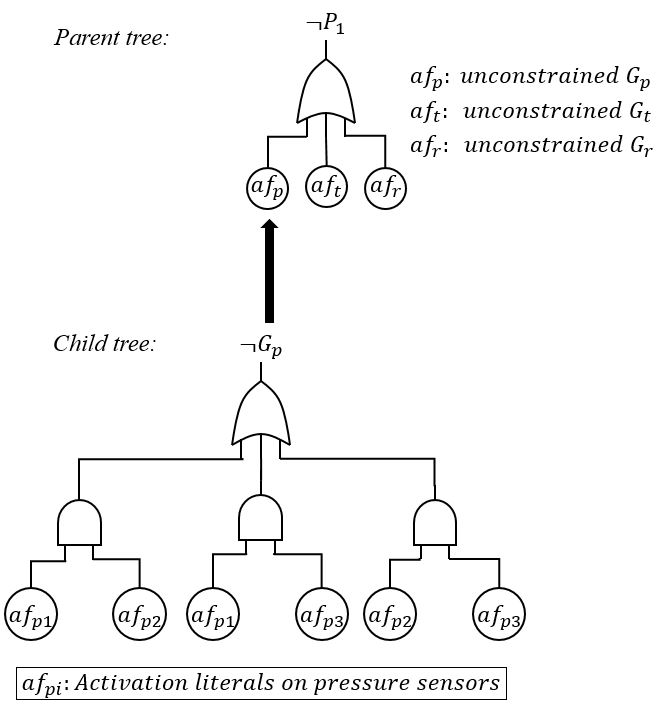
\includegraphics[width=0.5\textwidth]{images/faultCompEx.JPG}
	\end{center}
	\caption{Sensor System Composition of Fault Trees}
	\label{fig:sensorSysComp}
\end{figure}
We return to the sensor system example to illustrate this mapping. Graphically, this is represented in Figure~\ref{fig:sensorSysComp}.  The top level (parent) component is defined as: $\mathit{Comp}_p (M_p, \mathit{FF}_p, \mathit{NFV}_p, \pi_p)$ and $\mathit{FF}_p = \{(\neg P, \mathit{af}_p \lor \mathit{af}_t \lor \mathit{af}_r)\}$ where each activation literal is associated with the unconstrained guarantees $G_p$, $G_t$, and $G_r$. The child layer has a fault forest consisting of three fault trees, one for each subsystem. 

The pressure subsystem fault tree is $\mathit{FT}_{p} = (\neg G_p, (\mathit{af}_{p1} \land \mathit{af}_{p2}) \lor (\mathit{af}_{p1} \land \mathit{af}_{p3}) \lor (\mathit{af}_{p2} \land \mathit{af}_{p3}) $. The leaf formulae for each subsystem tree corresponds to pairwise combinations of active sensor faults. We now show the composition of the pressure subsystem child and top level parent fault trees. 

The mapping $\phi_F$ iterates through each tree in the parent forest -- in this case, we have only one. Then for each parent tree it iterates through the Boolean formulae in $\mathcal{L}$. If there is a match between a child root and a parent leaf, the replacement is made.
Thus, $\mathit{af}_p$ will be replaced with $(\mathit{af}_{p1} \land \mathit{af}_{p2}) \lor (\mathit{af}_{p1} \land \mathit{af}_{p3}) \lor (\mathit{af}_{p2} \land \mathit{af}_{p3})$. This replacement is done for each leaf formula in $\mathcal{L}_p$ from the parent fault forest. 

We represent the unconstrained (violated) guarantee as $\neg G_p$ and it is associated with the fault activation literal $\mathit{af}_p$. The end result of the replacement is easy to see.

%%%%5										COMPOSITION OF FF IS VALID
\begin{lemma} If $\mathit{FF}_c$ and $\mathit{FF}_p$ are valid fault forests, then their composition $\phi(\mathit{FF}_c, \mathit{FF}_p)$ is also a valid fault forest. 
\begin{proof}
By iterative application of Lemma~\ref{lemma:validTree}, the result is immediate.
\end{proof}
\label{lemma:validForest}
\end{lemma}

Thus far, we have proven that a single layer of composition produces valid fault trees (or forests), but to perform this analysis across $n$ layers of architecture we show inductively that the resulting fault forest is valid. 

The notation $\phi_F^n$ indicates the iterated function $\phi_F$ which is a successive application of $\phi_F$ with itself $n$ times. Assume the fault forest $\mathit{FF}_0$ is obtained at the leaf level of the architecture.

\begin{theorem} If $\phi_F^n(\mathit{FF}_{n-1}, \mathit{FF}_n)$ is a valid fault forest, then $\phi^{n+1}(\mathit{FF}_{n}, \mathit{FF}_{n+1})$ is a valid fault forest.
\begin{proof}

Base case: Each fault forest per layer is valid by construction. By Lemma~\ref{lemma:validForest}, $\phi_F(\mathit{FF}_{0}, \mathit{FF}_1)$ is a valid fault forest.

Inductive assumption: Assume $\phi_F^n(\mathit{FF}_{n-1}, \mathit{FF}_n)$ is a valid fault forest.
\begin{equation*}
\begin{split}
\phi_F^{n+1}(\mathit{FF}_{n}, \mathit{FF}_{n+1}) &= ((\mathit{FF}_0 \circ \mathit{FF}_1) \circ \mathit{FF}_2) \circ \cdots \circ \mathit{FF}_n) \circ \mathit{FF}_{n+1})) \\
  &= \phi_F^n(\mathit{FF}_{n-1}, \mathit{FF}_n) \circ \mathit{FF}_{n+1}
\end{split}
\end{equation*}

%$\phi_F^{n+1}(\mathit{FF}_{n}, \mathit{FF}_{n+1}) = ((\mathit{FF}_0 \circ \mathit{FF}_1) \circ \mathit{FF}_2) \circ \cdots \circ \mathit{FF}_n) \circ \mathit{FF}_{n+1})) = \phi_F^n(\mathit{FF}_{n-1}, \mathit{FF}_n) \circ \mathit{FF}_{n+1}$. 

By inductive assumption and Lemma~\ref{lemma:validForest}, $\phi_F^{n+1}(\mathit{FF}_{n}, \mathit{FF}_{n+1})$ is a valid fault forest.

\end{proof}
\label{thm:indForest}
\end{theorem}

We know from previous work that composition is conservative. A valid monolithic analysis of the transition system implies that the compositional analysis of that same system is valid, but the converse may not be true~\cite{}. It is likewise the case for composing fault forests. 

Let $S \subseteq \mathit{AF}$ where all $\mathit{af} \in S$ are constrained to true. If $S \cup \{\neg P\}$ is satisfiable, this equates to a valid fault tree. 

\begin{theorem} If $(I,T) \vdash P$ for monolithic verification, then for $S \subseteq \mathit{AF}$, $S \cup \{\neg P\}$ is unsatisfiable.
\begin{proof}
Assume toward contradiction that $(I,T) \vdash P$ and there exists a set $S \subseteq \mathit{AF}$ such that $S \cup \{\neg P\}$ is satisfiable. This implies that there exists a reachable state such that $\neg P$ holds. This contradicts our assumption. 
\end{proof}
\label{thm:sound}
\end{theorem}

As a counterexample to the converse of Theorem~\ref{thm:sound}, consider the following. \danielle{Counterexample here.}

Now that we have the formal foundations laid, we proceed towards the implementation. 






\section{Preliminaries for the Implementation}
\label{sec:prelim}

%%\textbf{Background Information on Toolsuite}
\danielle{My suggestion is to place this at the front of the implementation section. It just seems like it is taking longer to get to the interesting part of the paper by having it here.}

The algorithms in this paper are implemented in the Safety Annex for the Architecture Analysis and Design Language (AADL) and require the Assume-Guarantee Reasoning Environment (AGREE)~\cite{NFM2012:CoGaMiWhLaLu} to annotate the AADL model in order to perform verification using the back-end model checker \jkind~\cite{2017arXiv171201222G}. 

\textbf{Architecture Analysis and Design Language}
We are using the Architectural Analysis and Design Language (AADL) to construct system architecture models of performance-critical, embedded, real-time systems~\cite{AADL_Standard,FeilerModelBasedEngineering2012}. %An AADL model describes a system in terms of a hierarchy of components and their interconnections, where each component can either represent a logical entity (e.g., application software functions, data) or a physical entity (e.g., buses, processors). 
Language annexes to AADL provide a richer set of modeling elements for various system design and analysis needs, and the language definition is sufficiently rigorous to support formal analysis tools that allow for early phase error/fault detection. 

\textbf{Compositional Analysis} 
One way to structure compositional verification is hierarchically: layers of the system architecture are analyzed independently and their composition demonstrates a system property of interest. Compositional verification partitions the formal analysis of a system architecture into verification tasks that correspond into the decomposition of the architecture~\cite{clarke1989compositional}.  A proof consists of demonstrating that the system property is provable given the contracts of its direct subcomponents and the system assumptions~\cite{cofer2012compositional,clarke1989compositional}. When compared to monolithic analysis (i.e., analysis of the flattened model composed of all components), the compositional approach allows the analysis to scale to much larger systems~\cite{NFM2012:CoGaMiWhLaLu,heckel1998compositional,cofer2012compositional}.

\textbf{Assume Guarantee Reasoning Environment}
The Assume Guarantee Reasoning Environment (AGREE) is a tool for formal analysis of behaviors in AADL models and supports compositional verification~\cite{NFM2012:CoGaMiWhLaLu}.  It is implemented as an AADL annex and is used to annotate AADL components with formal behavioral contracts. Each component's contracts includes assumptions and guarantees about the component's inputs and outputs respectively. AGREE translates an AADL model and the behavioral contracts into Lustre~\cite{Halbwachs91:IEEE} and then queries the \jkind model checker to conduct the back-end analysis~\cite{2017arXiv171201222G}. 

\textbf{JKind}
JKind is an open-source industrial infinite-state inductive model checker for safety properties~\cite{2017arXiv171201222G}. Models and properties in JKind are specified in Lustre~\cite{Halbwachs91:IEEE}, a synchronous dataflow language, using the theories of linear real and integer arithmetic. JKind uses SMT-solvers to prove and falsify multiple properties in parallel.

\textbf{Safety Annex for AADL}
The Safety Annex for AADL provides the ability to reason about faults and faulty component behaviors in AADL models~\cite{Stewart17:IMBSA,stewart2020safety}. In the Safety Annex approach, AGREE is used to define the nominal behavior of system components, faults are introduced into the nominal model, and JKind is used to analyze the behavior of the system in the presence of faults. Faults describe deviations from the nominal behavior and are attached to the outputs of components in the system.%The Safety Annex supports behavioral specification of faults and their implicit propagation through behavioral relationships in the model as well as explicit propagation through dependencies. 
To implement the formalism described in Section~\ref{sec:formalization}, we must compute minimal cut sets per layer of analysis, transform them into their related Boolean formula, and compose them. As previously described, Ghassabani et al. developed the \textit{all minimal inductive validity core} algorithm (\aivcalg)~\cite{GhassabaniGW16,Ghassabani2017EfficientGO,bendik2018online}. The \aivcalg algorithm gives the minimal set of contracts required for proof of a safety property. If all of these sets are obtained, we have insight into every proof path for the property. Thus, if we violate at least one contract from every MIVC set, we have in essence ``broken" every proof. 
\begin{figure}[h!]
	\begin{center}
		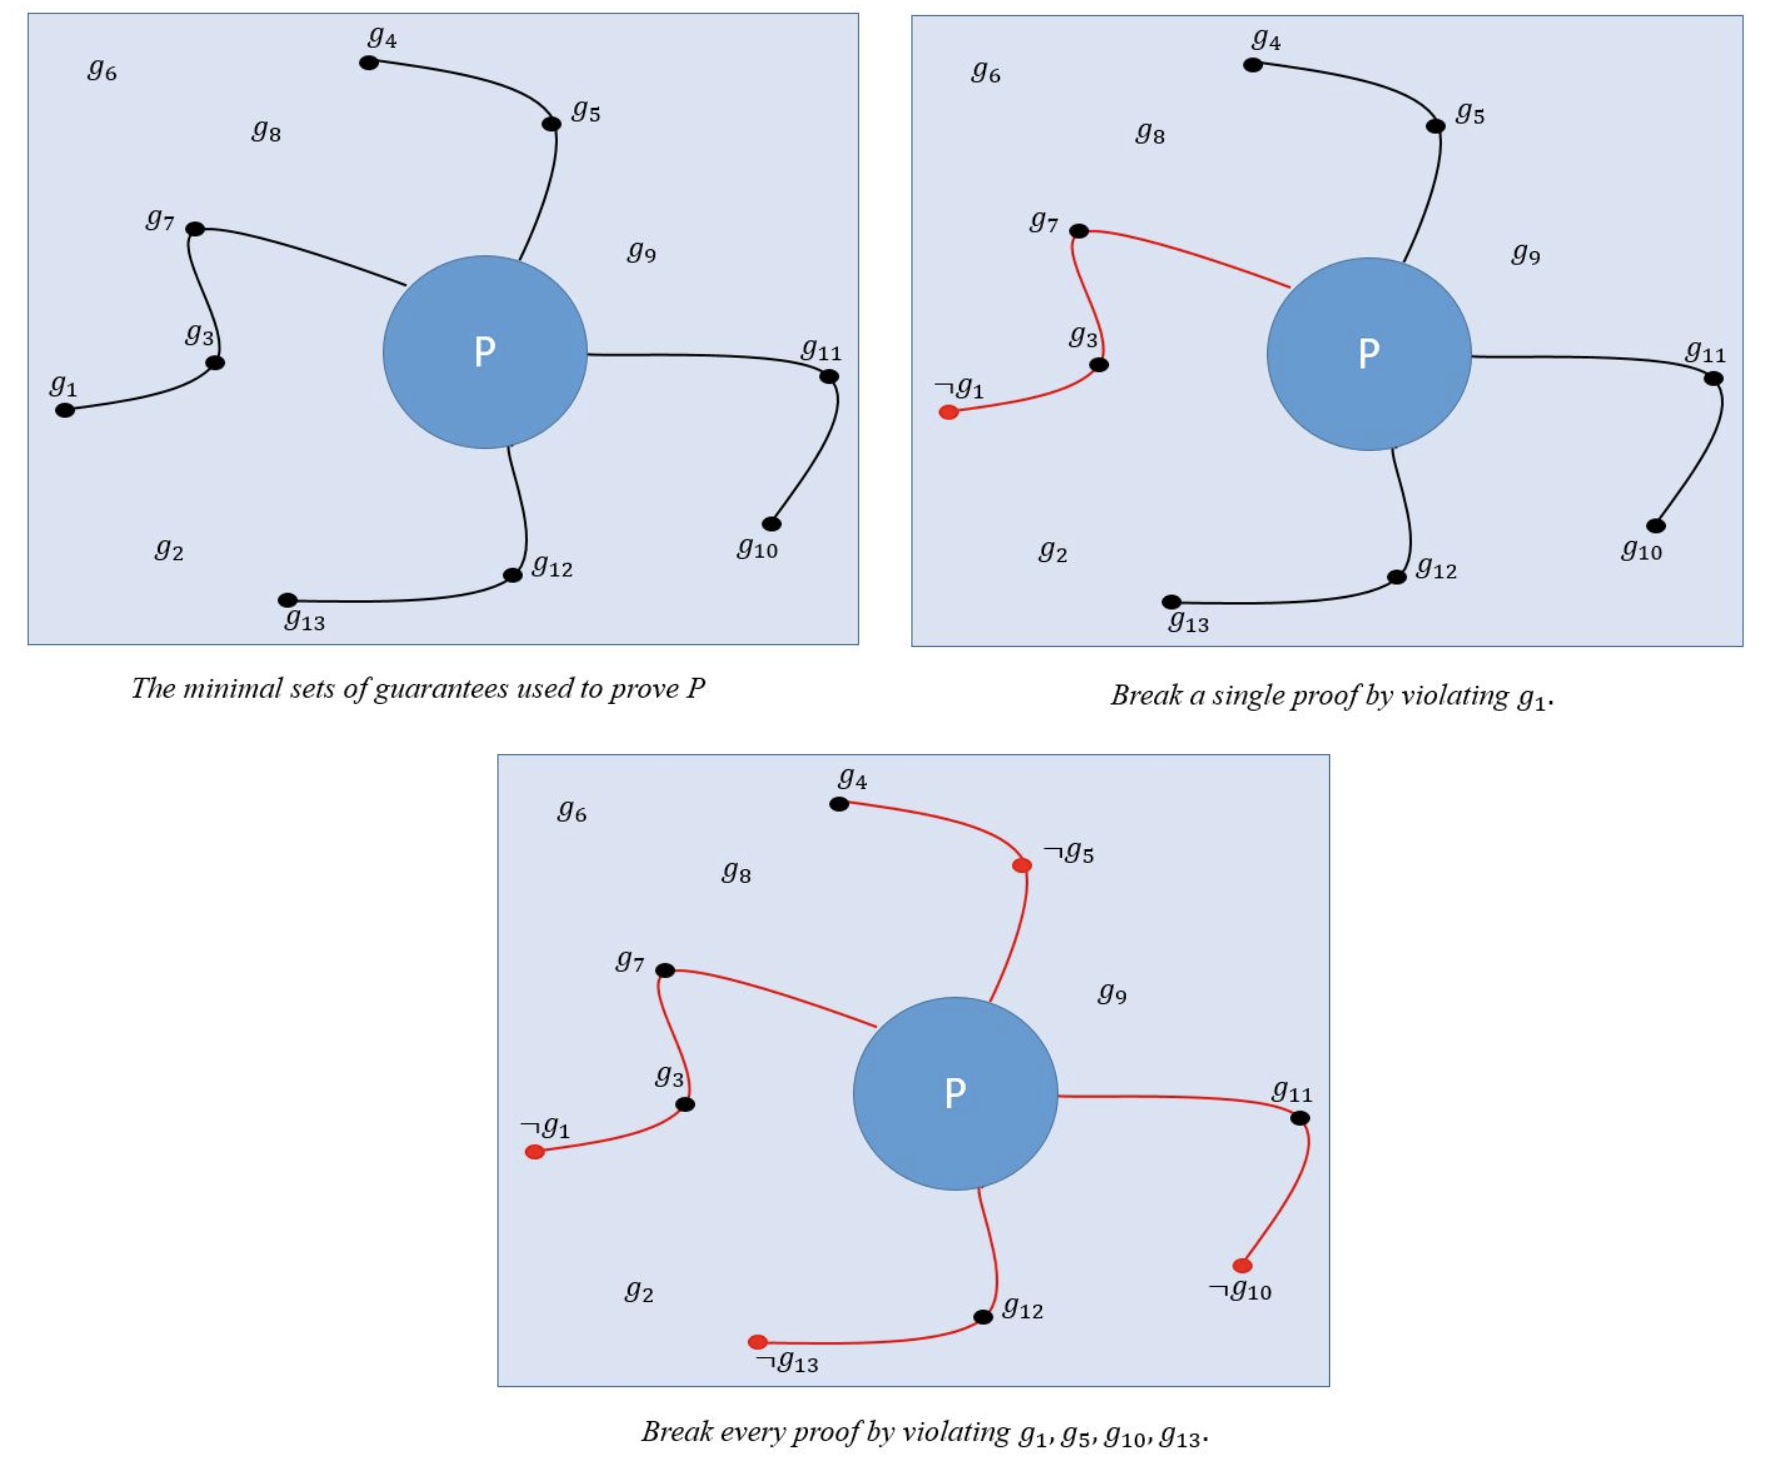
\includegraphics[width=0.9\textwidth]{images/mivcBreaking.png}
	\end{center}
	\caption{Using MIVCs to derive minimal cut sets}
	\label{fig:mivcBreaking}
\end{figure}

In Figure~\ref{fig:mivcBreaking}, we depict this graphically. In the first box (top left), the contracts of the single layer system are $g_1, \dots, g_{13}$. In this example, not all guarantees are needed to prove $P$; one may obtain proof of the property by having only $g_4$ and $g_5$ in the model. The \aivcalg algorithm provides all minimal validity cores which is shown as the lines running through the guarantees. 

One may attempt to ``break" a proof by violating a guarantee in a single MIVC as shown in the top right of the figure. This does break a proof, but given there are multiple MIVCs, it is not enough. The bottom figure shows our method: violate one guarantee from each MIVC set to ensure that the property can no longer be proven. The key idea is that the hitting sets of all MIVCs produces the minimal cut sets. 

Next we outline the formal background and toolsuite used in the implementation and then describe the algorithm that is implemented in the safety annex for AADL. 

\subsection{Background}
JKind is an open-source industrial infinite-state inductive model checker for safety properties~\cite{2017arXiv171201222G}. Models and properties in JKind are specified in Lustre~\cite{Halbwachs91:IEEE}, a synchronous dataflow language, using the theories of linear real and integer arithmetic. JKind uses SMT-solvers to prove and falsify multiple properties in parallel. The JKind model checker uses {\em
  $k$-induction} which unrolls the property $P$ over $k$ steps of the
transition system.

\begin{comment}
%For an arbitrary transition system $(I, T)$, computing reachability can be very expensive or even impossible. Thus, we need a more effective way of checking if a safety property $P$ is satisfied by the system. The key idea is to over-approximate reachability. If we can find an over-approximation that implies the property, then the property must hold. Otherwise, the approximation needs to be refined.

A good first approximation for reachability is the property itself.
That is, we can check if the following formulas hold:
\begin{gather}
  \forall s.~ I(s) \Rightarrow P(s)
  \label{eq:1-ind-base} \\
  \forall s, s'.~ P(s) \land T(s, s') \Rightarrow P(s')
  \label{eq:1-ind-step}
\end{gather}
If both formulas hold then $P$ is {\em inductive} and holds over the
system. If (\ref{eq:1-ind-base}) fails to hold, then $P$ is violated
by an initial state of the system. If (\ref{eq:1-ind-step}) fails to
hold, then $P$ is too much of an over-approximation and needs to be
refined.


The JKind model checker uses {\em
  $k$-induction} which unrolls the property $P$ over $k$ steps of the
transition system. For example, 1-induction consists of formulas (\ref{eq:1-ind-base}) and (\ref{eq:1-ind-step}) above, whereas 2-induction consists of the following formulas:
\begin{gather*}
\forall s.~ I(s) \Rightarrow P(s) \\
\forall s, s'.~ I(s) \land T(s, s') \Rightarrow P(s') \\
\forall s, s', s''.~ P(s) \land T(s, s') \land P(s') \land T(s',
  s'') \Rightarrow P(s'')
\end{gather*}
That is, there are two base step checks and one inductive step check.
In general, for an arbitrary $k$, $k$-induction consists of $k$
base step checks and one inductive step check as shown in
Figure~\ref{fig:k-induction} (the universal quantifiers on $s_i$ have
been elided for space). We say that a property is $k$-inductive if it
satisfies the $k$-induction constraints for the given value of $k$.
The hope is that the additional formulas in the antecedent of the
inductive step make it provable.

\begin{figure}
\begin{gather*}
I(s_0) \Rightarrow P(s_0) \\[-2pt]
%
\vdots \\[2pt]
%
I(s_0) \land T(s_0, s_1) \land \cdots \land T(s_{k-2}, s_{k-1})
\Rightarrow P(s_{k-1}) \\[2pt]
%
P(s_0) \land T(s_0, s_1) \land \cdots \land P(s_{k-1}) \land
T(s_{k-1}, s_k) \Rightarrow P(s_k)
\end{gather*}
\caption{$k$-induction formulas: $k$ base cases and one inductive
  step}
\label{fig:k-induction}
\end{figure}

In practice, inductive model checkers often use a combination of the
above techniques. Thus, a typical conclusion is of the form ``$P$ with
lemmas $L_1, \ldots, L_n$ is $k$-inductive''.
\end{comment}

Each step of induction is sent to an SMT (Satisfiabilty Modulo Theory)-solver to check for \emph{satisfiability}, i.e. there exists a total truth assignment to a given formula that evaluates to true. If there does not exist such an assignment, the formula is considered \emph{unsatisfiable}. %A \emph{constraint system} is a term used to describe the formula with all constraints to the variables. 
A $\mathit{k}$-induction model checker utilizes parallel SMT-solving engines at each induction step to glean information about the proof of a safety property. The transition formula is translated into clauses such that satisfiability is preserved~\cite{een2003temporal}. Expression of the base and induction steps of a temporal induction proof as SAT problems is straightforward and is shown below for step $k$:

\begin{gather*}
I(s_0) \land T(s_0, s_1) \land \cdots \land T(s_{k-1}, s_{k})
\land \neg P(s_{k})
\end{gather*}

When proving correctness it is shown that the formulas are \emph{unsatisfiable}, i.e., the property $P$ is provable. The idea behind finding an {\em inductive validity core} (IVC) for a given property $P$~\cite{GhassabaniGW16} is based on inductive proof methods used in SMT-based model checking, such as $\mathit{k}$-induction and IC3/PDR~\cite{een2011efficient, kahsai2012incremental, cook1971complexity}. Generally, an IVC computation technique aims to determine, for any subset $S \subseteq T$, whether $\mathit{P}$ is provable by $\mathit{S}$. A minimal subset that satisfies $\mathit{P}$ is seen as a minimal proof explanation and called a minimal inductive validity core. %Ghassabani et al. demonstrate that the minimization process is as hard as model checking~\cite{Ghassabani2017EfficientGO}, so finding a minimal inductive validity core may not be possible for some model checking problems. 

\begin{definition}
Inductive Validity Core (IVC)~\cite{GhassabaniGW16}: $S \subseteq T$ for $(I, T) \vdash P$ is an Inductive Validity Core, denoted by $\mathit{IVC(P,S)}$, iff $\mathit{(I,S)} \vdash P$.
\end{definition}

\begin{definition}
Minimal Inductive Validity Core (MIVC)~\cite{Ghassabani2017EfficientGO}: $S \subseteq T$ is a minimal Inductive Validity Core, denoted by $\mathit{MIVC(P,S)}$, iff $\mathit{IVC(P,S)} \land \forall T_i \in S$. $(I, S \setminus \{T_i\}) \not \vdash P$.
\end{definition}

The {\em constraint system} consists of the constrained formulas of the transition system and the negation of the property. The \aivcalg algorithm collects all {\em minimal unsatisfiable subsets} (MUSs) of a constraint system generated from a transition system at each induction step~\cite{Ghassabani2017EfficientGO,bendik2018online}. 

\begin{definition}
A Minimal Unsatisfiable Subset (MUS)~\cite{reiter1987theory} $M$ of a constraint system $C$ is a set $M \subseteq C$ such that $M$ is unsatisfiable and $\forall c \in M$ : $M \setminus \{c\}$ is satisfiable.
\end{definition}
The MUSs are the minimal explanation of the infeasibility of this constraint system; equivalently, these are the minimal sets of model elements necessary for proof of the safety property.

Returning to our running example, this can be illustrated by the following. Given the constraint system $C = \{G_p, G_t, G_r, \neg P\}$, a minimal explanation of the infeasability of this system is the set $\{G_p, G_t, G_r,\}$. If all three guarantees hold, then $P$ (the disjunction of these guarantees) is provable. 

In the case of an UNSAT system, we may ask: what will correct this unsatisfiability? A related set answers this question: 
\begin{definition}
A Minimal Correction Set (MCS)~\cite{reiter1987theory} $M$ of a constraint system $C$ is a subset $M\subseteq C$ such that $C \setminus M$ is satisfiable and $\forall M' \subset M$ : $C \setminus M'$ is unsatisfiable.
\end{definition}
A MCS can be seen to ``correct'' the infeasability of the constraint system by the removal from $C$ the constraints found in an MCS. Returning to the PWR example, the MCSs of the constraint system $C$ are $\mathit{MCS}_1 = \{G_t\}$, $\mathit{MCS}_2 = \{G_p\}$, $\mathit{MCS}_3 = \{G_r\}$. If any single guarantee is violated, a shut down from that subsystem may not get sent when it should and the safety property $P$ will be violated. This corresponds exactly to the definition of a minimal cut set.

For the following definitions, we remind readers of the extended transition system defined in Equation 2 of Section~\ref{sec:formalization} and that the elements of $T$ are the set $\mathit{GF} \cup \mathit{AF}$ for potentially faulty guarantees $\mathit{GF}$ and activation literals $\mathit{AF}$. We use the notation $\mathit{af} \rightarrow \{\mathit{true}, \mathit{false}\}$ to indicate a constraint on the literal $\mathit{af}$. 

\begin{definition}
A cut set $S$ of a top level event $\neg P$ is a set $S \subseteq \mathit{AF}$ such that $\forall \mathit{af} \in S$, $\mathit{af} \rightarrow \{\mathit{true}\}$ and $S \cup \{\neg P\}$ is satisfiable.
\end{definition}

Intuitively, a cut set is a true valuation for some subset of fault activation literals within a constraint system such that the constraint system is satisfiable given those true valuations.

\begin{definition}
A cut set $S$ is minimal if and only if $\forall \mathit{af} \in S$, $S \setminus \{\mathit{af}\} \cup \{\neg P\}$ is unsatisfiable.
\end{definition}

Our approach in computing minimal cut sets through the use of inductive validity cores is to supply activation literals constrained to be false to the algorithm. The resulting $\mathit{MCS}s$ consist of elements $\neg \mathit{af}_i$. The removal of this constraint from the constraint system results in non-deterministically true activation literals. By the definition of an $\mathit{MCS}$, we know that $C \setminus \mathit{MCS}$ is satisifiable. This removal of constraints from $C$ removes the {\em false} constraint from each element in the $\mathit{MCS}$. Liffiton et. al showed that any subset of a satisfiable set is also satisfiable~\cite{liffiton2016fast}, so we know that for set $S$ consisting of elements of $\mathit{MCS}$ with constraints removed, $S \cup \{\neg P\}$ is also satisfiable. This is the definition of a cut set. Minimality comes directly from the definition of a minimal correction set. 

A duality exists between the MUSs of a constraint system and the MCSs as established by Reiter \cite{reiter1987theory}. This duality is defined in terms of \textit{Minimal Hitting Sets} (\textit{MHS}). 
\begin{definition}
A hitting set of a collection of sets $A$ is a set $H$ such that every set in $A$ is ``hit'' by $H$; $H$ contains at least one element from every set in $A$. 
\end{definition}
Every MUS of a constraint system is a minimal hitting set of the system's MCSs, and likewise every MCS is a minimal hitting set of the system's MUSs. This is noted in previous work~\cite{liffiton2016fast, de1987diagnosing} and the proof of such is given by Reiter (Theorem 4.4 and Corollary 4.5)~\cite{reiter1987theory}. For the PWR top level constraint system, it can be seen that each of the MCSs intersected with the MUS is nonempty. This gives the minimal set of guarantees for which, if violated, will cause $P$ to be violated. 

As described in Section~\ref{sec:formalization}, we extend the transition system with fault activation literals. These literals are constrained to {\em false} and the \aivcalg algorithm is invoked. The constraint system for the PWR example is $C = \{\neg\mathit{af}_p, \neg\mathit{af}_t, \neg\mathit{af}_r, \neg P\}$ for activation literal $\mathit{af}_p$ associated with $G_p$, etc. The hitting sets generated from the MIVC are: $\{\neg\mathit{af}_p\}$, $\{\neg\mathit{af}_t\}$, and $\{\neg\mathit{af}_r\}$ and are the minimal correction sets of the constraint system. 

%\textbf{Background Information on Toolsuite}
\danielle{My suggestion is to place this at the front of the implementation section. It just seems like it is taking longer to get to the interesting part of the paper by having it here.}

The algorithms in this paper are implemented in the Safety Annex for the Architecture Analysis and Design Language (AADL) and require the Assume-Guarantee Reasoning Environment (AGREE)~\cite{NFM2012:CoGaMiWhLaLu} to annotate the AADL model in order to perform verification using the back-end model checker \jkind~\cite{2017arXiv171201222G}. 

\textbf{Architecture Analysis and Design Language}
We are using the Architectural Analysis and Design Language (AADL) to construct system architecture models of performance-critical, embedded, real-time systems~\cite{AADL_Standard,FeilerModelBasedEngineering2012}. %An AADL model describes a system in terms of a hierarchy of components and their interconnections, where each component can either represent a logical entity (e.g., application software functions, data) or a physical entity (e.g., buses, processors). 
Language annexes to AADL provide a richer set of modeling elements for various system design and analysis needs, and the language definition is sufficiently rigorous to support formal analysis tools that allow for early phase error/fault detection. 

\textbf{Compositional Analysis} 
One way to structure compositional verification is hierarchically: layers of the system architecture are analyzed independently and their composition demonstrates a system property of interest. Compositional verification partitions the formal analysis of a system architecture into verification tasks that correspond into the decomposition of the architecture~\cite{clarke1989compositional}.  A proof consists of demonstrating that the system property is provable given the contracts of its direct subcomponents and the system assumptions~\cite{cofer2012compositional,clarke1989compositional}. When compared to monolithic analysis (i.e., analysis of the flattened model composed of all components), the compositional approach allows the analysis to scale to much larger systems~\cite{NFM2012:CoGaMiWhLaLu,heckel1998compositional,cofer2012compositional}.

\textbf{Assume Guarantee Reasoning Environment}
The Assume Guarantee Reasoning Environment (AGREE) is a tool for formal analysis of behaviors in AADL models and supports compositional verification~\cite{NFM2012:CoGaMiWhLaLu}.  It is implemented as an AADL annex and is used to annotate AADL components with formal behavioral contracts. Each component's contracts includes assumptions and guarantees about the component's inputs and outputs respectively. AGREE translates an AADL model and the behavioral contracts into Lustre~\cite{Halbwachs91:IEEE} and then queries the \jkind model checker to conduct the back-end analysis~\cite{2017arXiv171201222G}. 

\textbf{JKind}
JKind is an open-source industrial infinite-state inductive model checker for safety properties~\cite{2017arXiv171201222G}. Models and properties in JKind are specified in Lustre~\cite{Halbwachs91:IEEE}, a synchronous dataflow language, using the theories of linear real and integer arithmetic. JKind uses SMT-solvers to prove and falsify multiple properties in parallel.

\textbf{Safety Annex for AADL}
The Safety Annex for AADL provides the ability to reason about faults and faulty component behaviors in AADL models~\cite{Stewart17:IMBSA,stewart2020safety}. In the Safety Annex approach, AGREE is used to define the nominal behavior of system components, faults are introduced into the nominal model, and JKind is used to analyze the behavior of the system in the presence of faults. Faults describe deviations from the nominal behavior and are attached to the outputs of components in the system.%The Safety Annex supports behavioral specification of faults and their implicit propagation through behavioral relationships in the model as well as explicit propagation through dependencies. 



\section{Implementation}
\label{sec:impl}
%%%%%%%%%%%%%%%%%%%%%%%%%%%%%%%%%%%%%%%%%%%%%%%%%
%%%%%%%%%%%%%%%%%%%%            ALGORITHM DETAILS
%In the formalism section, we viewed the problem from the perspective of an arbitary guarantee in the model that can potentially be violated. This resulted in explicit faults at the leaf level and violated guarantees (``nondeterministic faults") at the middle/top layers. Each MCS generated at each level gives insight into the system at that level. In this section, we describe the implementation of compositional generation of minimal cut sets. %Minimal cut sets traditionally contain explicitly defined faults as elements; to this end, we implemented a compositional mapping from explicit faults to the guarantees they violate. The end result are the minimal cut sets that contribute to a violation of the top level safety property. 
In the formalism, any guarantee in the model had an associated fault activation literal and could be unconstrained. In the implementation, we rely on the fault model created in the safety annex to dictate which guarantees can be violated and how they may fail. Each explicit fault defined in the safety annex is added to the Lustre program as are assocated fault activation literals~\cite{Stewart17:IMBSA,stewart2020safety}. This corresponds to the $f_i$ and $\mathit{af}_i$ described in Section~\ref{sec:formalization}. 

\begin{figure}[h!]
	%\vspace{-2em}
	\begin{center}
		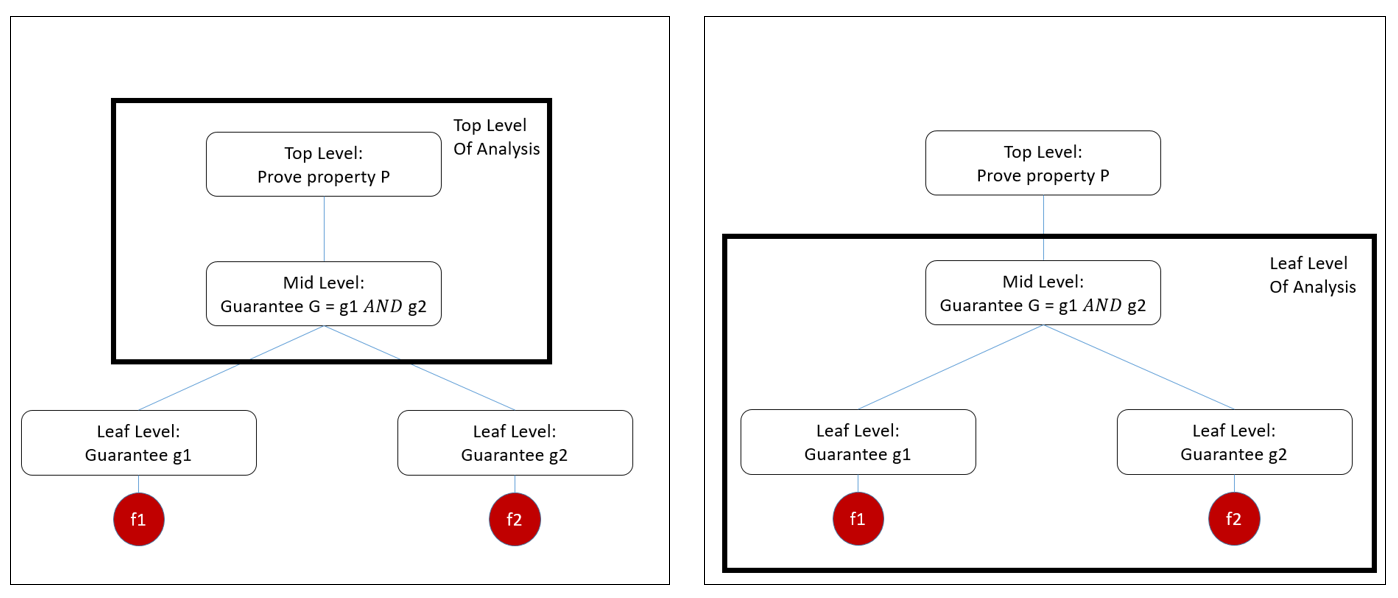
\includegraphics[width=0.9\textwidth]{images/twoLevels.PNG}
	\end{center}
	\vspace{-2em}
	\caption{Illustration of Two Layers of Analysis}
	\label{fig:layers}
\end{figure}

The \aivcalg algorithm requires  specific equations in the Lustre model to be flagged for consideration in the analysis; these we call \emph{IVC algorithm elements}. All equations in the model can be used as IVC algorithm elements or one can specify directly the equations to consider. In this implementation, the IVC algorithm elements are added differently depending on the layer. In the leaf architectural level, fault activation literals are added to the IVC algorithm elements and are constrained to {\em false}. In middle or top layers, supporting guarantees are added. This is shown in Figure~\ref{fig:layers}. 

The figure shows an arbitrary architecture with two analysis layers: top and leaf. The top layer analysis adds $G$ as IVC algorithm element; the leaf layer analysis adds $f_1$ and $f_2$. 

A requirement of the hitting set algorithm is that to find all MCSs, all MUSs must be known. Ghassabani et al.~\cite{Ghassabani2017EfficientGO} showed that finding all MIVCs is as hard as model checking. It is a requirement of this analysis that all MIVCs are found. Once the MIVC analysis is complete for a property at a given layer, a hitting set algorithm is used to generate the related MCSs~\cite{gainer2017minimal}. Depending on the layer of analysis, the MCSs contain either guarantees or fault activation literals.

%For a safety property $P$, the set of all MCSs are understood as $\lor^{n}_{i=1} MCS_i(P)$; intuitively, this means if all constraints found in any single MCS are removed from the constraint system, $\neg P$ is satisfied. For each element $gf_j \in MCS_i$, this is understood as $\land^{m}_{i=1} gf_i$ and speaks to the minimality of the correction set. Thus the MCSs form a disjunctive normal formula over the safety property at that layer. As the proof proceeds down the hierarchy, each of the subcomponent guarantees become a property to be proven and thus MIVCs/MCSs are generated. The composition of the MCSs consists of replacing a contract in a higher layer MCS with the disjunctive normal formula of its own MCSs. After all replacements have been made, the system property formula is converted back into disjunctive normal form. 

The composition of these results is performed top down and shown in Algorithm~\ref{alg:compose}. For each guarantee found in an MCS, a replacement is made with the guarantees own MCSs. This is done recursively until all replacements have been made (line 7, 8 of Algorithm~\ref{alg:compose}). If on the other hand there are no MCSs for a given guarantee, that guarantee is replaced by its associated fault activation literal (line 10). At the leaf level of analysis, no guarantees have associated MCSs and thus reaches the end of recursion. At that time, the formula is converted back into disjunctive normal form to finish the translation into the traditional fault tree (line 11). 

\begin{algorithm}[h]
\SetKwFunction{Resolve}{resolve}
 \SetKwProg{Fn}{Function}{:}{}

	$R \gets \mathit{\amcs(P)} = \lor_{i=1}^n \mathit{MCS}_i$\\
	where $\mathit{MCS}_i = \land_{j=1}^m \mathit{gf_j}$\\
	\Fn{\Resolve{$R$}}{
		
		\For{$\forall$ OR-node in $R$}{
			\For{$\forall \mathit{gf_j}$ in OR-node}{
				\eIf{ $\exists MCS(gf_j)$ }{
				$R \gets$ replace $gf_j$ in $R$ with $\mathit{\amcs(gf_j)}$\;
				\Resolve($\mathit{\amcs(gf_j)}$)\;
			}{
				$R \gets $ replace $\mathit{gf_j}$ in $R$ with $\mathit{af_j}$\;	
			} 
			}
		}
		convert $R$ to DNF 
	}
	\caption{Compose Results}
	\label{alg:compose}
\end{algorithm}

Algorithm~\ref{alg:compose} provides the outline for the general case of composing fault forests: for each each property in a layer, the algorithm is called. Each property may have a corresponding fault tree. The collection of fault trees associated with each property make the forest. In the next subsection, we describe how this general algorithm is adjusted.

\begin{comment}
The number of replacements $r$ that are made for a single property $P$ are constrained by the number of minimal cut sets there are for each of the $\alpha$ contracts within the initial MCS. We call the set of all minimal cut sets for a contract $g$: $\mathit{Cut(g)}$. The following formula defines an upper bound on the number of replacements. 

\begin{lemma}
The number of replacements $r$ is bounded by the following formula:
\begin{gather}
\label{eq:bound}
  r \leq {\displaystyle \sum_{i=1}^{\alpha} }({\displaystyle \prod_{j=1}^{i} |\mathit{Cut(g_j)}|})  
\end{gather}
\begin{proof}
Assume there exists a $g_i \in \mathit{MCS(P)}$. The number of replacements made for $g_i$ is at most $|\mathit{Cut(g_i)}|$. Iteratively perform this replacement for all $\alpha$ contracts in $\mathit{MCS(P)}$. In the worst case, $|\mathit{Cut(g_1)}| \times |\mathit{Cut(g_2)}| \times \cdots \times |\mathit{Cut(g_\alpha)}|$ replacements are made.
\label{lemma:bound}
\end{proof}
\end{lemma}

\end{comment}




\begin{theorem}
Algorithm~\ref{alg:compose} terminates
\begin{proof}
No infinite sets are generated by the \aivcalg or minimal hitting set algorithms~\cite{Ghassabani2017EfficientGO,murakami2013efficient}; therefore, every MCS produced is finite. Thus, every minimal cut set of every contract is finite.
\end{proof}
\end{theorem}

Given that the growth of the DNF formula can be exponential in the worst case, we implemented strategies to prune the size of the cut sets and hence the growth of these intermediate sets. 


\subsection{Pruning to Address Scalability}
The safety annex provides the capability to specify a type of verification in what is called a \textit{fault hypothesis statement}. These come in two forms: maximum number of faults or probabilistic analysis. Algorithm~\ref{alg:compose} is the general approach, but the implementation changes slightly depending on which form of analysis is being performed. This pruning improves performance and diminishes the problem of combinatorial explosion in the size of minimal cut sets for larger models. 

\textbf{Guarantees with no associated faults} If a guarantee is found in a minimal correction set and no fault has been defined in the model that can violate it, this minimal correction set (and hence the entire subtree) is pruned.

\textbf{Max $n$ faults analysis} The max $n$ fault hypothesis in the safety annex restricts the number of faults that can be independently active simultaneously. This statement restricts the cardinality of minimal cut sets generated to $n$. If the number of elements in an MCS exceeds the threshold of the hypothesis statement, that MCS is eliminated from consideration and its subtree is pruned.


\textbf{Probabilistic analysis pruning} A probabilistic hypothesis statement restricts the cut sets by use of a probabilistic threshold. Assuming independence between faults, any cut sets with combined probability higher than the given probabilistic threshold are removed from consideration. The allowable combinations of faults are calculated before Algorithm~\ref{alg:compose} begins; this allows for dynamic pruning of minimal correction sets. If the fault activation literals within an MCS are not a subset of any allowable combination, that MCS is pruned from the formula. 

To access the algorithm implementation or example models, see the repository~\cite{SAGithub}. 








\begin{comment}

\setcounter{AlgoLine}{0}
\Fn{\FindMIVCs{}}{
	\While{$\mathit{Unexplored} \neq \emptyset$}{
		%$U_{max} \gets$ a maximal $U_{max} \in \mathit{Unexplored}$\;
		$U_{\mathit{max}} \gets $ a maximal set $\in \mathit{Unexplored}$\;
        \eIf{$\Solve(I,U_{\mathit{max}},P)$}{
			$U_{\mathit{IVC}} \gets \approx((I,U_{\mathit{max}}), P)$\;
			$\Shrink(U_{\mathit{IVC}})$\;
		}{
			$\mathit{Unexplored} \gets \mathit{Unexplored} \setminus \mathit{Sub}(U_{\mathit{max}})$\;			
		}
		\While{$\mathit{shrinkingQueue}$ is not empty}{
			$\mathit{U} \gets \Dequeue(\mathit{shrinkingQueue})$\;
			$\Shrink(\mathit{U})$\;
		}
	}
}


The transformation of MIVCs to MinCutSets can only be performed if \emph{all} MIVCs have been generated. It is a requirement of the minimal hitting set algorithm that all MUSs are used to find the MCSs~\cite{liffiton2016fast,gainer2017minimal,murakami2013efficient}. Thus, once all MIVCs have been found and the minimal hitting set algorithm has completed, the MinCutSet generation can begin. 

The MinCutSet generation algorithm begins with a list of MCSs specific to a property. These MCSs may contain a mixture of fault activation literals constrained to \textit{false} and subcomponent contracts constrained to \textit{true}. We remove all constraints from each MCS and call the resulting sets $I$, for \textit{Intermediate} set.  For each of those contracts in $I$, we check to see if we have previously obtained a MinCutSet for that contract. If so, replacement is performed. If not, we recursively call this algorithm to obtain the list of all MinCutSets associated with this subcomponent contract. At a certain point, there will be no more contracts in the set $I$ in which case we have a minimal cut set for the current property. The reason is because at the lowest levels of the system, the only model elements used in the constraint system analyzed by the \aivcalg algorithm are faults. Thus when the contracts at the lowest level are the safety properties for the \aivcalg algorithm, the MUSs contain only faults (likewise the MCSs). When this cut set is obtained for the lowest level properties, it is stored in a lookup table keyed by the given property. Algorithm~\ref{alg:generation_alg} describes this process.


\begin{algorithm}[h]
\SetKwFunction{FMain}{replace}
 \SetKwProg{Fn}{Function}{:}{}

	\Fn{\FMain{$P$}}{
		$List(I)$:= $List(MCS)$ for $P$ with all constraints removed \;
		\For{all $I \in List(I)$}{
			\eIf{there exists contracts $g \in I$}{
				\For{all constrained contracts $g \in I$}{
					\eIf{there exists $MinCutSets$ for $g$ in lookup table}{
						\For{all $minCut(g)$}{
							$I_{repl} = I$ \;
							$I_{repl} :=$ replace $g$ with $minCut(g)$ \;
							add $I_{repl}$ to $List(I)$ \;
						} %end for all cut sets of g
					}{
						replace($g$) \;
					} % end else if no cut sets in lookup table
				} % end for all constrained contracts in I
			}{
				add $I$ as $minCut(g)$ for $P$ \;
			} %end else if there exists contracts in I
		}%end for all I in list(I)
	}
%	\caption{Minimal Cut Set Generation Algorithm}
	\caption{MinCutSets Generation Algorithm}
	\label{alg:generation_alg}
\end{algorithm}

The number of replacements $R$ that are made in this algorithm are constrained by the number of minimal cut sets there are for all $\alpha$ contracts within the initial MCS. 

We call the set of all minimal cut sets for a contract $g$: $Cut(g)$. The following formula defines an upper bound on the number of replacements. The validity of this statement follows directly from the general multiplicative combinatorial principle. The number of replacements $R$ is bounded by the following formula:
\begin{equation}
\label{eq:bound}
  R \leq {\displaystyle \sum_{i=1}^{\alpha} }({\displaystyle \prod_{j=1}^{i} |Cut(g_j)|})  
\end{equation}


It is also important to note that the cardinality of $List(I)$ is bounded, i.e. the algorithm terminates. Every new $I$ that is generated through some replacement of a contract with its minimal cut set is added to $List(I)$ in order to continue the replacement process for all contracts in $I$. Adding to this set requires proof regarding termination.
\begin{theorem}
Algorithm~\ref{alg:generation_alg} terminates
\begin{proof}
No infinite sets are generated by the \aivcalg or minimal hitting set algorithms~\cite{Ghassabani2017EfficientGO,murakami2013efficient}; therefore, every MCS produced is finite. Thus, every $MinCutSet$ of every contract $g$ is finite. Furthermore, a bound exists on the number of additional intermediate sets $I$ that are added to $List(I)$: \\
$|List(I)| \leq R$ (Equation~\ref{eq:bound}).
\end{proof}
\end{theorem}

The reason for this upper bound is that for a contract $g_1$ in MCS, we make $|Cut(g_1)|$ replacements and add the resulting lists to $List(I)$. Then we move to the next contract $g_2$ in $I$. We must additionally make $|Cut(g_1)| \times |Cut(g_2)|$ replacements and add all of these resulting lists to $List(I)$, and so on throughout all contracts. Through the use of basic combinatorial principles, we end with the above formula for the upper bound on the number of additional intermediate sets.


\subsubsection{Pruning to Address Scalability}
The MinCutSets are filtered during this process based on a fault hypothesis given before analysis begins. The Safety Annex provides the capability to specify a type of verification in what is called a \textit{fault hypothesis statement}. These come in two forms: maximum number of faults or probabilistic analysis. Algorithm~\ref{alg:generation_alg} is the general approach, but the implementation changes slightly depending on which form of analysis is being performed. This pruning improves performance and diminishes the problem of combinatorial explosions in the size of minimal cut sets for larger models. \\

\textbf{Max $N$ Analysis Pruning} This statement restricts the number of faults that can be independently active simultaneously and verification is run with this restriction present. For example, if a max 2 fault hypothesis is specified, two or fewer faults may be active at once. In terms of minimal cut sets, this statement restricts the cardinality of minimal cut sets generated.

If the number of faults in an intermediate set $I$ exceeds the threshold $N$, any further replacement of remaining contracts in that intermediate set can never decrease the total number of faults in $I$; therefore, this intermediate set is eliminated from consideration.\\

\textbf{Probabilistic Analysis Pruning} The second type of hypothesis statement restricts the cut sets by use of a probabilistic threshold. Any cut sets with combined probability higher than the given probabilistic threshold are removed from consideration. The allowable combinations of faults are calculated before the transformation algorithm begins; this allows for a pruning of intermediate sets during the transformation. If the faults within an intermediate set are not a subset of any allowable combination, that intermediate set is pruned from consideration and no further replacements are made. 

\end{comment}



\section{Related Work}
\label{sec:related_work}
Minimal cut sets generated by monolithic analysis look only at explicitly defined faults throughout the architecture and attempt through various techniques to find the minimal violating set for a particular property. We outline some of the common monolithic approaches to minimal cut set generation in this section.

The representation of Boolean formulae as Binary Decision Diagrams (BDDs) was first formalized in the mid 1980s~\cite{bryant1986graph} and were extended to the representation of fault trees not many years later~\cite{rauzy1993new}. After this formalization, the BDD approach to FTA provided a new approach to safety analysis. The model is constructed using a BDD, then a second BDD - usually slightly restructured - is used to encode MinCutSets~\cite{rauzy2008binary}. Unfortunately, due to the structure of BDDs, the worst case is exponential in size in terms of the number of variables~\cite{bryant1986graph,rauzy1993new,rauzy2008binary}. In industrial sized systems, this is not realistically useful. 

SAT based computation was then introduced to address scalability problems in the BDD approach; initially it was used as a preprocessing step to simplify the decision diagram~\cite{bozzano2015safety}, but later extended to allow for all MinCutSet processing and generation without the use of BDDs~\cite{bozzano2015efficient}. Since then, numerous safety related research groups have focused on leveraging the power of model checking in the problems of safety assessment~\cite{bieber2002combination,schafer2003combining,bozzano2007symbolic,bozzano2003improving,volk2017fast,Joshi05:SafeComp,bozzano2015efficient,stewart2020safety}. 

Bozzano et al. formulated a Bounded Model Checking (BMC) approach to the problem by successively approximating the cut set generation and computations to allow for an ``anytime approximation" in cases when the cut sets were simply too large and numerous to find~\cite{bozzano2015efficient,mattarei2016scalable}. These algorithms are implemented in xSAP~\cite{DBLP:conf/tacas/BittnerBCCGGMMZ16} and COMPASS~\cite{compass30toolset}. 

The model based safety assessment tool AltaRica 3.0~\cite{prosvirnova:tel-01119730} performs a series of processing to transform the model into a reachability graph and then compile to Boolean formula in order to compute the MinCutSets~\cite{prosvirnova2015automated}. Other tools such as HiP-HOPS~\cite{papadopoulos2001model} have implemented algorithms that follow the failure propagations in the model and collect information about safety related dependencies and hazards. The Safety Analysis Modeling Language (SAML)~\cite{Gudemann:2010:FQQ:1909626.1909813} provides a safety specific modeling language that can be translated into a number of input languages for model checkers in order to provide model checking support for MinCutSet generation.

To our knowledge, a fully compositional approach to calculating minimal cut sets has not been introduced.




















\section{Conclusion}

An extension to the AADL language has been developed with tool support for formal analysis of system safety properties in the presence of faults. Faulty behavior is specified as an extension of the nominal model, allowing safety analysis and system implementation to be driven from a single common model. This new Safety Annex leverages the AADL structural model and nominal behavioral specification (using the AGREE annex) to propagate faulty component behaviors without the need to add separate propagation specifications to the model.   Next steps will include extensions to automate injection of Byzantine faults as well as automatic generation of fault trees.  For more details on the tool, models, and approach, see the technical report and the repository~\cite{SATechReport, amaseRepo}.

\vspace{2 mm}
\noindent {\bf Acknowledgments.} This research was funded by NASA contract NNL16AB07T and the University of Minnesota College of Science and Engineering Graduate Fellowship.





%\vspace{-0.40cm}
\bibliographystyle{IEEEtran}

\bibliography{IEEEabrv,biblio}
%\vspace{-7.25cm}
% This ~ seems to fix an odd bibliography alignment issue


%\ifdefined\TECHREPORT
%\appendix
%
%\section{Appendix: Proof of Equivalence}
%\input{appendix}
%\fi

%\section{Appendix: GPCA CENTA Model}
%\label{appendix:gpcacenta}
%\begin{figure}[!ht]
%\begin{center}
%\includegraphics[scale=0.6]{images/sampled_pca.PNG} %[trim = 0 2 0 0, clip=true]{Comp}
%\caption{GPCA AGREE Properties modeled as a Timed Automata} \label{fig:samplepca}
%\end{center}
%\end{figure}

%\balancecolumns

\end{document} 